
%%%%%%%%%%%%%%%%%%%%%%%%%%%%%%%%%%%%%%%%%%%
%%%%%%%%%%%% BEHOLD THE %%%%%%%%%%%%%%%%%%%
%%%%%%%%%%%%  APPENDIX %%%%%%%%%%%%%%%%%%%%
%%%%%%%%%%%%%%%%%%%%%%%%%%%%%%%%%%%%%%%%%%%

\appendix
 


%%%%%%%%%%%%%%%%%%%%%%%%%%%%%%%%%%
\begin{comment}
\section{Terminology and Scope of Aggregate Neuronal Models} 

Under the umbrella of \emph{aggregate neuronal modeling} (also called \emph{neural mass}, \emph{population}, or \emph{lumped} models), we encompass a spectrum of formalisms that trade biological detail for analytical or computational simplicity.  This hierarchy can be traversed in both directions—adding realism to derive more mechanistic descriptions or stripping back complexity to reveal core dynamical principles:

\begin{itemize}
  \item \textbf{Phase oscillator:} describes the evolution of a single phase variable $\theta(t)$, capturing limit‐cycle interactions at the most abstract level.
  \item \textbf{Damped oscillator:} introduces amplitude relaxation, e.g., a second‐order linear system with friction.
  \item \textbf{Stuart–Landau (SL) normal form:} a generic nonlinear oscillator near a Hopf bifurcation, used phenomenologically to model neural rhythms.
  \item \textbf{Wilson–Cowan (WILCO):} the prototypical two‐population rate (population/lumped/neural‐mass) model, describing mean excitatory and inhibitory firing with coupled ODEs.
  \item \textbf{Neural Mass Model 1 (NMM1):} adds biophysical filtering of post‐synaptic potentials (PSPs) and explicit conversion from mean membrane potentials to firing rates.
  \item \textbf{Neural Mass Model 2 (NMM2 or MPR):} extends NMM1 by incorporating dynamics in the transfer function.
\end{itemize}

When we take the limit of infinitely many, infinitesimally small populations (or let the spatial coupling kernel become continuous), this lumped description generalizes to integro‐differential or partial‐differential equations known as \emph{neural field models}.


Aggregate neuronal models (phase oscillators, SL, WILCO, NMM1, NMM2, etc.) are fundamentally \emph{statistical constructs} that provide macro‐level, effective descriptions of complex networks of many neurons.  All share these core features:

\begin{enumerate}
  \item \emph{Mean variables:} each model tracks ensemble averages—phase and amplitude (phase oscillator, SL), firing rate (WILCO), membrane potential and PSP (NMM1), plus synchronization metrics (NMM2).
  \item \emph{Aggregation by type:} neurons are grouped into populations based on anatomical and functional characteristics, each treated as a single ``lumped'' unit.
  \item \emph{Effective parameters:} time‐constants, gains and connectivities summarize average behavior; they do not map one‑to‑one onto single‑cell properties.
  \item \emph{Scale invariance:} the dynamical equations predict the same trajectories regardless of neuron count, provided effective parameters (e.g. mean synapses per neuron) remain fixed.
  \item \emph{Bridge to measurements:} to relate outputs (phase, rate, or voltage) to LFP, current‐source density, or BOLD signals, morphological and density‐based scaling factors must be applied post‐hoc.
\end{enumerate}


\clearpage







%%%%%%%%%%%%%%%%%%%%%%%%%%%%%%%%%%%%%%%%%%%%
\section{Coordinate Transformations}
\label{sec:appendix_coord}

This appendix provides the full mathematical derivations of how one obtains Cartesian and complex representations from polar form (and vice versa) for both the undamped and damped oscillators.

\subsection{Undamped Oscillator: Polar $\longleftrightarrow$ Cartesian $\longleftrightarrow$ Complex}

\paragraph{Polar to Cartesian.}

Starting from the polar equations
\begin{align}
    \dot{\theta} &= \omega, 
    \label{eq:A_undamped_polar_theta}\\
    \dot{r}      &= 0,
    \label{eq:A_undamped_polar_r}
\end{align}
define 
\begin{equation}
    x = r \cos\theta, 
    \qquad
    y = r \sin\theta.
    \label{eq:A_xy_def}
\end{equation}
Differentiate $x$ and $y$ with respect to time.  Since $r=r_{0}$ is constant,
\begin{align*}
    \dot{x} 
    &= \frac{d}{dt}\bigl(r\cos\theta\bigr) 
     = -\,r\,\sin\theta \;\dot{\theta} 
     = -\,r\,\sin\theta\,(\omega) 
     = -\,\omega\,(r\sin\theta) 
     = -\,\omega\,y, \\[6pt]
    \dot{y} 
    &= \frac{d}{dt}\bigl(r\sin\theta\bigr) 
     = r\,\cos\theta \;\dot{\theta} 
     = r\,\cos\theta\,(\omega) 
     = \omega\,(r\cos\theta) 
     = \omega\,x.
\end{align*}
Hence,
\begin{equation}
    \dot{x} = -\,\omega\,y,
    \qquad
    \dot{y} = \omega\,x,
    \label{eq:A_undamped_cart}
\end{equation}
which recovers the undamped Cartesian form~\eqref{eq:undamped_cart_x}–\eqref{eq:undamped_cart_y}.

\paragraph{Cartesian to Complex.}

Given $x(t)$ and $y(t)$ satisfying~\eqref{eq:A_undamped_cart}, set
\begin{equation}
    z = x + i\,y.
    \label{eq:A_z_def}
\end{equation}
Then
\begin{align*}
    \dot{z} 
    = \dot{x} + i\,\dot{y} 
    = (-\,\omega\,y) + i\,(\omega\,x) 
    = i\,\omega\,(x + i\,y) 
    = i\,\omega\,z,
\end{align*}
recovering the undamped complex form~\eqref{eq:undamped_complex}.

Conversely, writing $z = r\,e^{\,i\,\theta}$ and differentiating yields
\[
    \dot{z} 
    = \dot{r}\,e^{\,i\,\theta} \;+\; r\,e^{\,i\,\theta}\,i\,\dot{\theta}
    = (\dot{r} + i\,r\,\dot{\theta})\,e^{\,i\,\theta}.
\]
By matching $\dot{z} = i\,\omega\,z = i\,\omega\,r\,e^{\,i\,\theta}$, one finds 
\[
    \dot{r} = 0, 
    \qquad
    \dot{\theta} = \omega,
\]
which recovers~\eqref{eq:A_undamped_polar_r}–\eqref{eq:A_undamped_polar_theta}.

\subsection{Damped Oscillator: Polar $\longleftrightarrow$ Cartesian $\longleftrightarrow$ Complex}

\paragraph{Polar to Cartesian.}

Begin with the damped polar equations:
\begin{align}
    \dot{r}      &= \alpha\,r \;+\; F_{r}(t), 
    \label{eq:A_damped_polar_r}\\
    \dot{\theta} &= \omega \;+\; \frac{F_{\theta}(t)}{r}.
    \label{eq:A_damped_polar_theta}
\end{align}
Define
\begin{equation}
    x = r \cos\theta, 
    \qquad
    y = r \sin\theta,
    \label{eq:A_damped_xy}
\end{equation}
and differentiate:
\[
    \dot{x} 
    = \dot{r}\,\cos\theta \;-\; r\,\sin\theta\,\dot{\theta},
    \qquad
    \dot{y} 
    = \dot{r}\,\sin\theta \;+\; r\,\cos\theta\,\dot{\theta}.
\]
Substitute $\dot{r}$ and $\dot{\theta}$ from~\eqref{eq:A_damped_polar_r}–\eqref{eq:A_damped_polar_theta}:
\begin{align*}
    \dot{x} 
    &= \bigl(\alpha\,r + F_{r}(t)\bigr)\cos\theta 
       \;-\; r\,\sin\theta \Bigl(\omega + \tfrac{F_{\theta}(t)}{r}\Bigr) \\[4pt]
    &= \alpha\,(r\cos\theta) \;+\; F_{r}(t)\cos\theta 
       \;-\; \omega\,(r\sin\theta) \;-\; \sin\theta\,F_{\theta}(t) \\[6pt]
    &= \alpha\,x \;-\; \omega\,y \;+\; \bigl[F_{r}(t)\cos\theta - F_{\theta}(t)\sin\theta\bigr].
\end{align*}
Similarly,
\begin{align*}
    \dot{y} 
    &= \bigl(\alpha\,r + F_{r}(t)\bigr)\sin\theta 
       \;+\; r\,\cos\theta \Bigl(\omega + \tfrac{F_{\theta}(t)}{r}\Bigr) \\[4pt]
    &= \alpha\,(r\sin\theta) \;+\; F_{r}(t)\sin\theta 
       \;+\; \omega\,(r\cos\theta) \;+\; \cos\theta\,F_{\theta}(t) \\[6pt]
    &= \alpha\,y \;+\; \omega\,x \;+\; \bigl[F_{r}(t)\sin\theta + F_{\theta}(t)\cos\theta\bigr].
\end{align*}
Define
\begin{equation}
    I_{x}(t) \;=\; F_{r}(t)\,\cos\theta \;-\; F_{\theta}(t)\,\sin\theta,
    \qquad
    I_{y}(t) \;=\; F_{r}(t)\,\sin\theta \;+\; F_{\theta}(t)\,\cos\theta.
    \label{eq:A_forcing_rel}
\end{equation}
Then
\begin{align}
    \dot{x} &= -\,\omega\,y \;+\; \alpha\,x \;+\; I_{x}(t), 
    \label{eq:A_damped_cart_x}\\
    \dot{y} &= \;\,\omega\,x \;+\; \alpha\,y \;+\; I_{y}(t),
    \label{eq:A_damped_cart_y}
\end{align}
which recover the damped Cartesian form~\eqref{eq:damped_cart_x}–\eqref{eq:damped_cart_y}.

\paragraph{Cartesian to Complex.}

From~\eqref{eq:A_damped_cart_x}–\eqref{eq:A_damped_cart_y}, let $z = x + i\,y$ and $I_{z}(t) = I_{x}(t) + i\,I_{y}(t)$.  Then
\begin{align*}
    \dot{z} 
    &= \dot{x} + i\,\dot{y} \\
    &= \bigl(-\,\omega\,y + \alpha\,x + I_{x}(t)\bigr) 
       + i\,\bigl(\omega\,x + \alpha\,y + I_{y}(t)\bigr) \\[4pt]
    &= \alpha\,(x + i\,y) \;+\; i\,\omega\,(x + i\,y) \;+\; (I_{x} + i\,I_{y}) \\[4pt]
    &= (\alpha + i\,\omega)\,z \;+\; I_{z}(t),
\end{align*}
yielding the damped‐and‐forced complex form~\eqref{eq:damped_complex}.

Conversely, writing $z = r\,e^{\,i\,\theta}$,
\[
    \dot{z} 
    = \dot{r}\,e^{\,i\,\theta} + i\,r\,\dot{\theta}\,e^{\,i\,\theta} 
    = \bigl(\dot{r} + i\,r\,\dot{\theta}\bigr)\,e^{\,i\,\theta}.
\]
Matching $\dot{z} = (\alpha + i\,\omega)\,z + I_{z}(t) = (\alpha + i\,\omega)\,r\,e^{\,i\,\theta} + I_{z}(t)$, one identifies
\begin{align*}
    \dot{r}         &= \alpha\,r \;+\; \Re\bigl(e^{-\,i\,\theta} I_{z}(t)\bigr), \\[4pt]
    r\,\dot{\theta} &= \omega\,r \;+\; \Im\bigl(e^{-\,i\,\theta} I_{z}(t)\bigr),
\end{align*}
so that, by defining $F_{r}(t) = \Re(e^{-\,i\,\theta} I_{z}(t))$ and $F_{\theta}(t) = \Im(e^{-\,i\,\theta} I_{z}(t))$, one recovers the polar form~\eqref{eq:A_damped_polar_r}–\eqref{eq:A_damped_polar_theta}.

\bigskip
\noindent\textbf{Notation and Labels in Appendix:}
\begin{itemize}
    %\item Equations in the appendix are labeled with an ``A'' prefix (e.g.,~\eqref{eq:A_undamped_cart}, \eqref{eq:A_damped_cart_x}).
    \item The external inputs $I_{x}(t),I_{y}(t)$ in Cartesian form are related to radial/tangential forcings $F_{r}(t),F_{\theta}(t)$ via~\eqref{eq:A_forcing_rel}.
    \item The complex input $I_{z}(t)$ is $I_{x}(t) + i\,I_{y}(t)$.
\end{itemize}


\subsection{WILCO and second order equations}

Unlike phase–amplitude models that admit a natural polar form, the Wilson-Cowan system 
is most naturally expressed in a 2D \((x,y)\) phase plane. We can interpret
\[
\mathbf{X} \;=\; \begin{pmatrix} x \\[4pt] y \end{pmatrix},
\quad
\dot{\mathbf{X}}
\;=\;
\begin{pmatrix}
\dot{x}\\[4pt]
\dot{y}
\end{pmatrix},
\]
and rewrite the Wilson-Cowan equations in vector form:
\[
\begin{pmatrix}
\tau_x\,\dot{x}\\[2pt]
\tau_y\,\dot{y}
\end{pmatrix}
=
\begin{pmatrix}
-\,x + S_{x}(w_{xx}\,x - w_{xy}\,y + I_x)\\[4pt]
-\,y + S_{y}(w_{yx}\,x - w_{yy}\,y + I_y)
\end{pmatrix}.
\]
Phase‐plane analysis (nullclines, fixed points, and limit cycles) is used to study 
how \(\mathbf{X}\) evolves in \(\mathbb{R}^2\).


\paragraph{Second order equations.}
Because each equation is second-order, one can rewrite them as pairs of first--order
ODEs. For instance, let \(x_1 = x\) and \(x_2 = \dot{x}\). Then:
\[
\begin{cases}
\dot{x}_1 = x_2,\\[6pt]
\dot{x}_2 = \displaystyle \frac{1}{\tau_x^2}\Bigl[
-\,2\tau_x\,x_2 \;+\; K_{x}\,S_{x}\bigl(\cdots\bigr) \;-\; x_1
\Bigr].
\end{cases}
\]
Similarly for \((y_1,y_2)\). Alternatively, one may keep the original form and 
perform phase--space analysis in four dimensions \((x,\dot{x},y,\dot{y})\).
The \(-\,x\) and \(-\,y\) terms (right--hand side) act as a linear decay, while
the second--order operator allows for resonant or damped oscillatory responses 
that are further modulated by the nonlinear saturations \(S_{x}\) and \(S_{y}\).
%%%%%%%%%%%%%
\clearpage

\end{comment}





%%%%%%%%%%%%%%%%%%%%%%%%%%%%%%%%%%%%%%%%%%%%%%%%%%
\clearpage 

%%%%%%%%%%%%%%%%%%%%%%%%%
\clearpage
\section{Linear Stability and Bifurcation Analysis}
\label{sec:bifurcations}
\begin{comment}\subsection{Linear stability analysis}
A feature that all neural mass models discussed in main text have in common, except for the harmonic oscillator, is that they are all nonlinear models. Although most nonlinear systems are impractical to solve analytically and the use of numerical methods are often required, we can still gain insights in the systems behaviors through linearization methods. As the literature in this topic is very rich, we will briefly review main concepts that will help the reader understand the dynamical behavior of the neural mass models discussed in the main text.

First, is it worth to recall that a $N$-dimensional linear system, which can be written as
\begin{equation}
    \dot{\mathbf{x}}(t) =\begin{bmatrix}
        a_{11} & a_{12} & ... & a_{1N} \\
        a_{21} & a_{22} & ... & a_{2N} \\
        \vdots & \vdots & \ddots & \vdots \\
        a_{N1} & a_{N2} & ... & a_{NN} \\        
    \end{bmatrix}
    \begin{bmatrix}
        x_1(t) \\
        x_2(t) \\
        \vdots \\
        x_N(t)
    \end{bmatrix}
    = A \mathbf{x}(t)
\end{equation}
Notice that at each instant $t$ the matrix $A$ \emph{linearly} transforms the vector $\mathbf{x}$. To obtain the solution of this systems we can rely on the fact that $A$ can be diagonalized, hence it can be expressed as:
\begin{equation}
     A = P \Lambda P^{-1}
\end{equation}
where $P$ is the matrix whose columns are the eigenvectors of $A$, and $\Lambda$ is the diagonal matrix whose entries are the eigenvalues $\{\lambda_i\}$ of $A$. 
Substituting we have
\begin{equation}
\mathbf{\dot x} = P \Lambda P^{-1}\mathbf{x}(t) \ .
\end{equation}
Introducing $\mathbf{z}(t) = P^{-1}\mathbf{x}(t)$, we have
\begin{equation}
\dot{\mathbf{z}}(t) = \Lambda\mathbf{z}(t) =
        \begin{bmatrix}
        \lambda_1 z_1(t) \\
        \lambda_2 z_2(t) \\
        \vdots \\
        \lambda_N z_N(t)
    \end{bmatrix} \ .
\end{equation}
And have a solution of the form $z_i(t) = c_i e^{\lambda_i t}$, thus
\begin{equation}
    \mathbf{z}(t) =
    \begin{bmatrix}
        c_1 e^{\lambda_1 t} \\
        c_2 e^{\lambda_2 t} \\
        \vdots \\
        c_N e^{\lambda_N t}
    \end{bmatrix} \ .
\end{equation}
Finally, using that $\mathbf{x}(t) = P\mathbf{z}(t)$, we get
\begin{equation}
\mathbf{x}(t) = c_1 e^{\lambda_1 t} \mathbf{v}_1 + c_2 e^{\lambda_2 t} \mathbf{v}_2 + \ldots + c_N e^{\lambda_N t} \mathbf{v}_N
\label{eq:linear_sol}
\end{equation}
where $\mathbf{v}_1, \mathbf{v}_2, \ldots, \mathbf{v}_N$ are the corresponding eigenvectors of $A$ and  $c_1, c_2, \ldots, c_N$ are constants determined by the initial conditions of the system. In this form, it is clear that the solution and hence the dynamics of the system will be dictated by its eigenvalues, which can be real or complex. For example, if we take a two-dimensional system with $c_i > 0$, we have
\begin{equation}
\mathbf{x}(t) = c_1 e^{\lambda_1 t} \mathbf{v}_1 + c_2 e^{\lambda_2 t} \mathbf{v}_2
\end{equation}
If both $\lambda_1$ and $\lambda_2$ are positive, the system diverges as both exponentials grow to infinity; on the other hand, if both are negative, the exponentials tend to zero. Notice how the magnitude of the eigenvalues will determine the speed with which the system evolves in each direction. Interestingly, if the eigenvalues form a complex conjugate, $\lambda_{1,2} = \alpha \pm i\beta$ which allow solutions of the type
\begin{equation}
\mathbf{x}(t) =  c_1 e^{(\alpha_1 \pm i\beta_1)t} +  c_2 e^{(\alpha_2 \pm i\beta_2)t} = c_1 e^{\alpha_1t}\cos(\beta_1t)\mathbf{v}_1 + c_2 e^{\alpha_2t}\cos(\beta_2t) \mathbf{v}_2   
\end{equation}
and hence oscillatory behavior.

Of special interest to us is the behavior of the system around \emph{fixed points} $\mathbf{x}^*$. Fixed points are defined by solutions to 
\begin{equation}
    \dot{\mathbf{x}}(t) = \mathbf{F}(\mathbf{x}) = 0
\label{eq:fixed_point}
\end{equation}
which represent equilibrium solutions, since if the system starts at $\mathbf{x}^*$, it will stay there if it is kept unperturbed.

Now, if we take a nonlinear system 
\begin{equation}
    \mathbf{\dot{x}} = \mathbf{F}(\mathbf{x})
\end{equation}
where $F$ represents a \emph{nonlinear} transformation of the vector $x$ and usually cannot be diagonalized, we can not obtain a solution with form of Eq. \eqref{eq:linear_sol}.
Fortunately, we can linearize nonlinear systems around their fixed points, which at first order yield us
\begin{equation}
    \mathbf{\dot{x}} \approx \mathbf{F}(\mathbf{x}^*) + D\mathbf{F}(x)|_{\mathbf{x}^*} (\mathbf{x}-\mathbf{x}^*) + \mathcal{O}^2 \ .
\end{equation}
And by using $\mathbf{F}(\mathbf{x}^*)=0$, discarding higher order terms we get:
\begin{equation}
    \mathbf{\dot{x}} \approx D\mathbf{F}(x)|_{\mathbf{x}^*} (\mathbf{x}-\mathbf{x}^*).
\end{equation}
This linear version of our original system, allow us to use the linear analysis tools to get an insight on the dynamical properties of the nonlinear system: the eigenvalues $\lambda$ of the Jacobian matrix $D\mathbf{F}$ will encoded the behavior of system around the fixed points.

Below, we summarize the different types of fixed points in Table \ref{table:fixed_points}. While we focus on two-dimensional systems for clarity, the reasoning applies to 
$N$-dimensional systems: the eigenvalues of the Jacobian still determine the local stability and type of equilibrium. The classification in higher dimensions, though, involves more combinations of stable, unstable, and center directions. Readers interested in the general case can consult standard references on nonlinear dynamics such as \cite{strogatz_nonlinear_2015,kuznetsov2023elements,datseris2022}.

While fixed points correspond to states where the system remains constant over time, some nonlinear systems exhibit limit cycles, in which the system evolves along a closed, repeating trajectory in phase space. \emph{Limit cycles} represent self-sustained oscillations and can be either stable, attracting nearby trajectories, or unstable, repelling them. In this way, limit cycles extend the concept of equilibrium from a single point to a periodic orbit. Their stability are encoded by \emph{Floquet exponents}.

Beyond understanding the local behavior around fixed points and limit cycles, it is equally important to study how changes in the system’s parameters affect its qualitative dynamics. Such transitions occur when fixed points (the solutions of Eq.~\eqref{eq:fixed_point}) or limit cycles appear, disappear, or change stability, typically reflected in changes in the sign or nature (real/complex) of their associated eigenvalues. These qualitative changes are known as \emph{bifurcations} and their analysis can be facilitated using bifurcation diagrams, which provide a clear visual representation of how the system’s behavior evolves as parameters vary.

\begin{table}[h!]
\centering
\caption{Classification of Fixed Points in 2D Linear Systems $\dot{\mathbf{x}} = A\mathbf{x}$}
\renewcommand{\arraystretch}{1.3}
\setlength{\tabcolsep}{5pt}
\begin{tabular}{p{3.5cm} p{3.5cm} p{2.5cm} p{6cm}}
\hline
\textbf{Eigenvalues $(\lambda_1, \lambda_2)$} &
\textbf{Type} &
\textbf{Stability} &
\textbf{Phase Portrait Description} \\
\hline
$\lambda_1, \lambda_2 > 0$ &
Unstable node (source) &
Unstable &
Trajectories move directly away from the origin. \\

$\lambda_1, \lambda_2 < 0$ &
Stable node (sink) &
Stable &
Trajectories move directly into the origin. \\

$\lambda_1 < 0 < \lambda_2$ &
Saddle point &
Unstable &
Attracted along one eigendirection and repelled along the other. \\

$\lambda_1 = \lambda_2 < 0$  &
Proper node (sink) &
Stable &
Straight-line approach to origin. \\

$\lambda_1 = \lambda_2 > 0$  &
Proper node (source) &
Unstable &
Straight-line repulsion from origin. \\

$\lambda = \alpha \pm i\beta, \ \alpha < 0$ &
Stable focus (spiral sink) &
Asymptotically stable &
Spirals inward toward the origin. \\

$\lambda = \alpha \pm i\beta, \ \alpha > 0$ &
Unstable focus (spiral source) &
Unstable &
Spirals outward from the origin. \\

$\lambda = \pm i\beta$ &
Center &
Neutrally stable &
Closed periodic orbits around the origin. \\
\hline
\end{tabular}
\label{table:fixed_points}
\end{table}

\end{comment}

\subsection{Bifurcation diagrams}

Bifurcation diagrams provide a powerful way to visualize how the qualitative behavior of a dynamical system changes as key parameters vary, and they are widely used to study the emergence of oscillatory dynamics. In this section, we discuss the common bifurcations observed in neural mass models by examining their bifurcation diagrams. We emphasize that these diagrams depend strongly on the chosen parameter values, and this section is not intended to serve as an exhaustive catalogue of all possible dynamical regimes. For comprehensive analyses of each model, we will refer the reader to the dedicated literature.

We focus on one-parameter bifurcation diagrams, which we compute using the AUTO-07p software package. This tool allows us to identify fixed points and limit cycles, along with their stability properties. The scripts used to generate all bifurcation diagrams presented here, along with a complete list of parameters, are available at \cite{doedel2007auto07p}.

\subsubsection*{Stuart-Landau}
We begin with the Stuart-Landau (SL) model, which is given by
\begin{align}
  \dot{x} &= \alpha\,x - \omega\,y
           - \gamma\,(x^{2}+y^{2})\,x
           + \beta\,(x^{2}+y^{2})\,y,
  \label{eq:sl_cart_x2}\\
  \dot{y} &= \alpha\,y + \omega\,x
           - \gamma\,(x^{2}+y^{2})\,y
           - \beta\,(x^{2}+y^{2})\,x,
\end{align}
Setting $\gamma = 1$ and $\beta = 0$, we get
\begin{align}
  \dot{x} &= \alpha\,x - \omega\,y
           - (x^{2}+y^{2})\,x
           ,
  \\
  \dot{y} &= \alpha\,y + \omega\,x
           - (x^{2}+y^{2})\,y
\end{align}
The bifurcation diagram of the later, using $\alpha$ as the bifurcation parameter, is shown in Fig. \ref{fig:SL_bif}. The dark (light) gray line represents the stable (unstable) fixed points. For $\alpha < 0$, the system has complex eigenvalues with negative real parts, meaning that trajectories spiral towards the fixed point (damped oscillations). For $\alpha > 0$, the real parts of the eigenvalues are positive, so trajectories are repelled from the fixed point and attracted to the stable limit cycle, with amplitude represented in blue. This transition, in which a fixed point changes its stability while a stable (or unstable) limit cycle emerges, is known as a supercritical (or subcritical) Hopf bifurcation, here referred to as HB$^{+(-)}$.
 


\rev{The bifurcation diagrams for the Wilson--Cowan and NMM1 (Jansen--Rit, Wendling, LaNMM) models, previously included here, have been moved into the main body of the paper---see~\S\ref{sec:WILCO} and~\S\ref{sec:NMM1}. The diagrams below cover the remaining models in the cross-walk, namely the next-generation NMM2 ING and PING motifs.}

\subsubsection*{ING}
Our analysis now shifts to NMM2 models. We start with the ING model with second-order synapses, whose dynamics are governed by the following system of equations: 
\begin{equation}
\begin{aligned}
\tau_i \dot{v} &= \eta - \left( \pi r \tau_m \right)^2 + v^2 - \tau_i \left( J_{ii} s \right) + I \\
\tau_i \dot{r} &= \Delta + 2 r v \\
\tau_g \dot{s} &= z \\
\tau_g \dot{z} &= r - 2z - s
\end{aligned}
\end{equation}
The bifurcation diagram for the NMM2 model of interneuron-gamma (ING) oscillations is shown in Fig.~\ref{fig:ING_bif}. It illustrates the steady-state firing rate $r$ as a function of the external input $I$. As in the previous models, increasing the external input induces a transition from a stable fixed point to oscillatory activity via a supercritical Hopf bifurcation (HB$^{+}$). The resulting limit-cycle oscillations persist over a range of input values and are terminated at a second HB$^{+}$, with both bifurcation points indicated by the vertical dashed lines.


\subsubsection*{PING}
We continue our analysis of the NMM2 family by shifting our attention to the PING model, which can be viewed as a natural extension of the ING framework. The governing equations of the PING system are given by
\begin{equation}
\begin{aligned}
\tau_e \dot{v}_e &= \eta_e - \left( \pi r_e \tau_e \right)^2 + v_e^2 + \tau_e \left( J_{ee} s_e - J_{ei} s_i \right) + I \\
\tau_e \dot{r}_e &= \Delta_e + 2 r_e v_e \\
\tau_a \dot{s}_e &= z_e \\
\tau_a \dot{z}_e &= r_e - 2z_e - s_e \\
\tau_i \dot{v}_i &= \eta_i - \left( \pi r_i \tau_i \right)^2 + v_i^2 + \tau_i \left( J_{ie} s_e - J_{ii} s_i \right) + I \\
\tau_i \dot{r}_i &= \Delta_i + 2 r_i v_i \\
\tau_g \dot{s}_i &= z_i \\
\tau_g \dot{z}_i &= r_i - 2z_i - s_i
\end{aligned}
\end{equation}
The bifurcation diagram of the PING model is shown in Fig.~\ref{fig:PING_bif}. It depicts the steady-state firing rate as a function of the external input ($I$). 
From left to right, as the external input increases, the system first undergoes a pair of saddle-node (SN) bifurcations, indicating the creation and annihilation of fixed points. Following these, the system experiences a supercritical Hopf bifurcation (HB$^{+}$), giving rise to stable oscillatory dynamics. The resulting limit-cycle oscillations persist over a range of input values until the system passes through another HB$^{+}$ bifurcation, at which the oscillations disappear and the system returns to a stable fixed point.



\newpage

To summarize, bifurcation diagrams are particularly valuable for neural mass models because they:

\begin{itemize}
    \item \textbf{Reveal the onset of oscillations and other dynamical regimes.}
    They identify where fixed points lose stability and give rise to limit cycles, as well as where bistability or other qualitative transitions occur, providing a clear picture of the model’s possible behaviors.

    \item \textbf{Guide parameter selection and sensitivity analysis.}
    By showing how solutions depend on parameters such as coupling strengths or synaptic gains, bifurcation diagrams help identify which parameters critically shape the dynamics and which regimes are physiologically plausible.

    \item \textbf{Inform control and intervention strategies.}
    In applications ranging from neuromodulation to pharmacology, knowing how small parameter changes can shift the system between regimes is essential. Bifurcation diagrams make these transitions explicit by highlighting where stability changes occur.
\end{itemize}
 

\clearpage

\begin{landscape}
\setlength{\LTcapwidth}{\textwidth}
{\small
\begin{longtable}{@{}llp{4.8cm}p{8cm}}
  \caption{Parameters used for the bifurcation diagram in
  this paper. The code to reproduce the diagrams using \texttt{AUTO-07P} is available at \url{https://github.com/pclus/auto-tutorial}.}
  \label{tab:bif-params}\\
  \toprule
  \textbf{Fig.} & \textbf{Panel} & \textbf{Swept parameter} &
  \textbf{Fixed parameters} \\
  \midrule
  \endfirsthead
  \multicolumn{4}{@{}l}{\textit{Table~\ref{tab:bif-params} continued}}\\
  \toprule
  \textbf{Fig.} & \textbf{Panel} & \textbf{Swept parameter} &
  \textbf{Fixed parameters} \\
  \midrule
  \endhead
  \midrule
  \multicolumn{4}{r}{\textit{continued on next page\ldots}}\\
  \endfoot
  \bottomrule
  \endlastfoot


% --- Other models ---
  \multicolumn{4}{@{}l}{\textit{Stuart--Landau}}\\
  Fig.~\ref{fig:SL_bif} & --- & $\alpha\in[-10,10]$ & $\omega=1$ \\ \midrule
  
  % --- Wilson--Cowan ---
  \multicolumn{4}{@{}l}{\textit{Wilson--Cowan}}\\
  \addlinespace[2pt]
  Fig.~\ref{fig:wilco_two_personalities} & (a) & $P_x\in[-5,5]$  &
   $\kappa_{xx}$ = $\kappa_{xy}=\kappa_{yx}=12$, $\kappa_{yy}=2$, $\tau_x = \tau_y = 1$, $\rho=1$, $\theta_x = \theta_y = 0$, $e_0 = 1$, $P_y=-6$ \\
    & (b) & $P_y\in[-10,0]$  \& same as (a) except for $I_x=0$ & \\
  \midrule
  \multicolumn{4}{@{}l}{\textit{Jansen--Rit}}\\
  Fig.~\ref{fig:JR_bif} & --- & $P\in[-80,350]$ & Same parameters as in \cite{JansenRit1995} and \cite{GrimbertFaugeras2006} \\ \midrule
  \multicolumn{4}{@{}l}{\textit{Wendling}}\\
  Fig.~\ref{fig:Wend_bif} & --- & $P\in[0,1700]$ & Same parameters as in \cite{wendlingEpilepticFastActivity2002} \\ \midrule
  \multicolumn{4}{@{}l}{\textit{LaNMM} }\\
  Fig.~\ref{fig:LaNMM_bif} & --- & $P\in[-100,500]$ & Same parameters as in \cite{sanchez-todoPhysicalNeuralMass2023} and \cite{depalmaaristidesEmergenceMultifrequencyActivity2025}\\ \midrule
  \multicolumn{4}{@{}l}{\textit{NMM2-ING} }\\
  Fig.~\ref{fig:ING_bif} & --- & $I\in[-20,100]$ & $\eta=0$, $J_{ii}=20$, $\tau_i=7.5$, $\tau_g = 2$, $\Delta=1$ \\ \midrule
  \multicolumn{4}{@{}l}{\textit{NMM2-PING}}\\
  Fig.~\ref{fig:PING_bif} & --- & $I\in[-20,75]$ & $\eta_e=\eta_i=0$, $J_{ee}=J_{ei}=J_{ie}=1$, $J_{ii}=2$,  $\tau_e = 15, \tau_a=10$, $\tau_i = 7.5, \tau_g = 2.5$, $\Delta_e=\Delta_i=1$\\
\end{longtable}
}
\end{landscape}
%%%%%%%%%%%%%%%%%%%%%%%%%%%%%%%%%%%%%%%%%%%
\begin{comment}\clearpage
\section{Phase dynamics and Kuramoto model}
\label{app:kuramoto}
In the main text, we begin with a pure phase oscillator model and gradually introduce increasing mathematical complexity.
Nonetheless, coupled phase oscillator models, particularly the Kuramoto model, were originally derived from arbitrary oscillator 
systems subject to weak perturbations by employing rigorous mathematical techniques.
Such approach, usually known as \emph{phase reduction}, was pioneered by Winfree and Kuramoto,
 and has been widely applied in mathematical neuroscience to capture the phase dynamics of both single-neuron and neural population models. For a comprehensive treatment of these methods, readers may refer to~\cite{Winfree2001,Kuramoto1984,hoppensteadt1997,Pikovsky2003}.
 Drawing on this literature, in this Appendix we provide a concise introduction to the phase reduction technique in a general setting, and then illustrate it using the Stuart–Landau oscillator, which naturally leads to the Kuramoto model.

\subsection{Phase of a perturbed oscillator}
\label{app:phase_of_perturbed_oscillator}
% PHASE OF A LIMIT-CYCLE
Let us consider an $m$-dimensional variable $\bs{x}\in\mathbb{R}^m$, whose time evolution is ruled by the differential equation
\begin{equation}\label{introeq:system}
\dot{\bs{x}}=\bs{\mathcal {F}}(\bs{x})
\end{equation}
where $\bs{\mathcal{F}}$ is a smooth function. Let us assume that equation~(\ref{introeq:system})
has an attracting limit-cycle with period $T$, $\bs {x}_{\text{LC}}(t)=\bs {x}_{\text{LC}}(t+T)$.
Thus, the curve $\bs{x}$ is, by definition, parameterized by time, $t\in[0,T)$.
We define the \emph{phase} of a point $\bs{x}(t)$ of $\bs x_{\text{LC}}$ as
\begin{equation}
\phi(\bs x(t)):=t\frac{2\pi}{T}\in[0,2\pi).
\end{equation}
For simplicity, we denote $\omega:=\frac{2\pi}{T}$.\\

% ISOCHRONES
The concept of phase is well defined for any point lying exactly on the limit cycle.
Nevertheless, the phase reduction approach is based on extending the notion of phase to a neighborhood $G\subset \mathbb{R}^m$ of $\bs x_{\text{LC}}(t)$.
Let $\bs y_0=\bs y(0)\in\mathbb{R}^m$ be a point in the state space close to, but not exactly on the periodic attractor $\bs x_{\text{LC}}$.
Since the limit cycle is stable, the trajectory $\bs y(t)$ will end up arbitrarily close to $\bs x_{\text{LC}}$ as $t\to\infty$,
thus will have a well defined phase, $\phi(\bs y(t))$.
Therefore, even if $\bs y_0$ is not on the invariant manifold,
one can find a point, $\bs x_0\in \bs x_{\text{LC}}$ such that, at long-term,
$\phi(\bs y(t))=\phi(\bs x(t))$.
One can then define the phase of $\bs y_0$ as $\phi(\bs y_0)=\phi(\bs x_0)$.
All the points in the neighborhood of $\bs x_{\text{LC}}$ associated to the same phase form a \emph{isochrone curve},
i.e., the isochrones are the level curves of the function $\phi$.
\\

This extension of the notion of phase to the vicinity of the periodic orbit preserves a constant time evolution:
\begin{equation}\label{introeq:phaseoscillator}
\dot \phi(\bs x)=\omega\;, \qquad \bs x \in G.
\end{equation}
Applying the chain rule and using Eq.~\ref{introeq:system}, one obtains
\begin{equation}
\dot \phi(\bs x)=\grad_{\bs x} \phi \cdot \bs{\mathcal{F}}(\bs x).
\end{equation}
Combining the two previous equations provides
\begin{equation}\label{introeq:phaseequality}
\grad_{\bs x} \phi \cdot \bs{\mathcal{F}}(\bs x)=\omega\;.
\end{equation}
This equation expresses then, that the variation of the phase under the effect of the field $\bs{\mathcal{F}}$
is constant.

% PHASE RESPONSE CURVE
We want to study oscillatory systems that are interacting with a certain environment, so, usually,
equation~(\ref{introeq:system}) is not enough for our purposes. One needs to
account for the effect that external perturbations have on the system.
Let us assume a perturbation on the evolution of $\bs x$, $\bs p(t)$, with a small amplitude parameter $ 0<\varepsilon \ll 1$,
\begin{equation}
 \dot{\bs{x}}=\bs{\mathcal {F}}(\bs{x})+\varepsilon \bs{p}(t).
\end{equation}
In order to keep arguing in terms of phases, one needs to find which is the impact of
such perturbation on the phase of the oscillator.
Applying again the chain rule to the time evolution of $\phi$, and using Eq.~(\ref{introeq:phaseequality}) one obtains
\begin{align}
\dot \phi(\bs x)
&=\grad_{\bs x}\phi \cdot \left(\bs{\mathcal{F}}(\bs x)+\varepsilon \bs p(t)\right) \\
&=\omega+\varepsilon \grad_{\bs x}\phi\cdot \bs p(t) \label{introeq:winfree}
\end{align}
Thus, as one would expect, the linear response of the phase $\phi$ to a perturbation of the trajectory is given by its gradient.
For this reason, the gradient of the phase along a certain unitary direction $\bs{\delta x}$ is usually referred to as the \emph{Phase Response Curve} (PRC), $Z(\phi):=\grad_{\bs { x}}\phi \cdot \bs {\delta x}$.
Following the definition of gradient, given a infinitesimal  perturbation $\varepsilon \bs{\delta x}$ of a point on the limit cycle $\bs x$,
 one can effectively compute the phase response curve as the normalized difference between the phase of $\bs {x}$,
 and that of $\bs{x}+\varepsilon \bs{\delta x}$,
\begin{equation}
Z(\phi)=\frac{ \phi(\bs x)-\phi(\bs{ x}+\varepsilon\bs{\delta x}) }{\varepsilon  }\;.
\end{equation}
Thus, a positive (resp. negative) PRC indicates that the perturbation has the effect of advancing (resp. delaying) the phase of the oscillator.
A zero PRC means that the perturbed point lies exactly on the isochrone of the original point.
For simplicity, on the following we assume that the perturbation $\bs p(t)$ has direction $\bs {\delta x}$ and modulus $p(t)$ so that
$\grad_{\bs x}\phi\cdot \bs p(t)=Z(\phi) p(t)$. Thus, Eq~(\ref{introeq:winfree}) now reads
\begin{equation}\label{introeq:winfree2}
\dot \phi(\bs x)=\omega + \varepsilon Z(\phi)p(t)\;.
\end{equation}
Systems with this form are known as \emph{Winfree-type models} of phase oscillators~\cite{Winfree2001},
where the PRC, $Z(\phi)$, and the shape of the forcing $\bs p(t)$ are defined independently one from the other.

\subsection{From Winfree to Kuramoto}

Let's assume now the phase dynamics of two interacting oscillators of Winfree type:
\begin{align}\label{introeq:winfree3}
\dot \phi_1 &= \omega_1 + \varepsilon Z(\phi_1)g(\phi_2)\\
\dot \phi_2 &= \omega_2 + \varepsilon Z(\phi_2)g(\phi_1)\;.
\end{align}
Notice that now the forcing term $p(t)$ has been replaced by a $2\pi$-periodic interaction function $g(\phi)$.
It is possible to further simplify this system by separating time scales on the dynamics of the phase model.
Since $\varepsilon\ll 1$ in Eq.~(\ref{introeq:winfree3}), one expects that the changes
in the evolution of $\phi_j$ mostly happen at a slow time scale, since the fast dynamics is
driven by the natural frequency of oscillation $\omega_j$.
Let's study then the time evolution of the slow variables $\varphi_j=\phi_j-\omega_j t$.
With this change of variables, equation~(\ref{introeq:winfree3}) now reads
\begin{equation}
\dot \varphi_j=   \varepsilon Z(\varphi_j-\omega_j t)g(\varphi_k-\omega_k t)\;.
\end{equation}
In order to retain the terms relevant for the evolution of $\varphi_j$ one can expand
the previous equation in Fourier series,
\begin{align}\label{introeq:tokuramoto}
\dot \varphi_j=   \varepsilon  Z(\varphi_j-\omega_j t)g(\varphi_k-\omega_k t)
        &=\frac{\varepsilon}{4\pi^2}\sum_{m,n}\tilde Z(m)\tilde p(n)e^{-i[m(\varphi_j-\omega_j t) +n(\varphi_k-\omega_k t)]}\\
        &=\frac{\varepsilon}{4\pi^2}\sum_{m,n}\tilde Z(m)\tilde p(n)e^{-im(\varphi_j-\varphi_k)}e^{i(m\omega_j + n\omega_k)t}\;.
\end{align}
The last expression provides a separation of the fast and slow terms in the series:
the terms with
\begin{equation}
 m\omega_j +n \omega_k \simeq 0
\end{equation}
are resonant, and, therefore, lead to slow dynamics.
The other terms, instead, have explicit dependence on $t$, and, therefore, lead to rapid changes.
Thus, in order to keep only the relevant dynamics of the system, one can average out
the non-resonant terms.
Under the assumption that the natural frequencies of the two oscillator are comparable, \emph{i.e.}, $\omega_j\simeq \omega_k$,
the terms of Eq.~(\ref{introeq:tokuramoto}) relevant for the dynamics are those with
$m=-n$.
This leads to
\begin{equation}
    \dot \varphi_j=   
         =\frac{\varepsilon}{4\pi^2}\sum_{n=-\infty}^\infty\tilde Z(-n)\tilde p(n)e^{-in(\varphi_k-\varphi_j)}=H(\varphi_j-\varphi_k) 
\end{equation}
where the \emph{coupling function} $H$ can be computed as
\begin{equation}
H(\psi):=\frac{1}{4\pi^2}\sum_{n=-\infty}^\infty \tilde Z(-n)\tilde p(-n)e^{-in \psi}
=\frac{1}{2\pi}\int_0^{2\pi} Z(t)p(t+\psi) dt.
\end{equation}
Writing now system~(\ref{introeq:winfree3}) into the original variables, we finally obtain:
\begin{align}\label{introeq:phasemodel}
\dot \phi_1&=\omega_1+\varepsilon H(\phi_2 -\phi_1)\\
\dot \phi_2&=\omega_2+\varepsilon H(\phi_1 -\phi_2)\;.
\end{align}
Phase oscillators ruled by equations of this type are known as \emph{Kuramoto-Daido type} models.
Despite their simplicity, such systems provide a good framework
to study emerging phenomena on networks of oscillators.
The simplest of these models corresponds to $H$ being composed of a single harmonic, i.e.,
$$H(\psi) = \sin(\psi-\alpha),$$
leading to the famous Kuramoto-Sakaguchi model. 
Nonetheless, the phase reduction of most nonlinear oscillators contain more harmonics in their 
coupling function, which usually also increase the complexity of the model dynamics.

Here, we provided a simple intuitive arguments on how the time-scale separation is being performed.
Formally, the coupling function $H$ emerges from applying averaging theory to system \eqref{introeq:winfree3}.
% COMMENT ON "ORDER EPSILON" AND "HIGHER ORDER INTERACTIONS".
These rigorous derivations also allow to extend this approach to more complex situations, including
an arbitrary number of oscillators, 
cases in which the interaction function $g$ depends on both, pre and post-synaptic units, $g(\phi_1,\phi_2)$,
and cases with other resonant relation between the units. 
Nonetheless, here we want to emphasize the two main assumptions that allow to obtain Kuramoto-Daido models
from arbitrary limit cycles: weak coupling ($\varepsilon\ll 1$), and weak frequency heterogeneities ($\omega_1\approx \omega_2$). 

\subsection{Phase reduction of a Stuart-Landau system}

In general, performing the phase reduction of a nonlinear oscillator requires a numerical approach.
Due to its simplicity and symmetry properties, the Stuart-Landau oscillator is a notable exception.
Here we reproduce a well-known result that a system of coupled Stuart-Landau oscillators
leads to the Kuramoto-Sakaguchi model:
\begin{equation}
\dot{z}_{i} = (\alpha + i\,\omega_{i})\,z_{i}
             - (\gamma + i\,\beta)\,\lvert z_{i}\rvert^{2}z_{i}
             + \frac{\varepsilon}{N}\sum_{j=1}^{N}\bigl(z_{j}-z_{i}\bigr)\;.
\end{equation}

Let's first determine the phase variable of an uncoupled oscillator.
We work using the polar representation:
\begin{align}
  \dot{r}      &= \alpha\,r \;-\; \gamma\,r^{3},\\
  \dot{\theta} &= \omega \;-\; \beta\,r^{2}.
\end{align}
The system contains an (unstable) fixed point at $r=0$.
For any other initial condition, $r(0)=r_0\neq 0$ and $\theta(0)=\theta_0$, the solution of the system reads:
\begin{equation}
    r(t) = \sqrt{\frac{\alpha}{\gamma + \left(\frac{\alpha}{r_0^2}-\gamma\right)e^{-2\alpha t}}}
    \qquad
    \theta(t) = \omega - \frac{\alpha\beta}{\gamma} +\theta_0 
    - \frac{\beta}{2\gamma} \ln\left[ \frac{\gamma}{\alpha} r_0^2 + e^{-2\alpha t}\left(1-\frac{\gamma}{\alpha}r_0^2 \right)\right]\;. 
\end{equation}
As $t\to\infty$ the equation evolves towards a limit cycle with amplitude $r_* = \sqrt{\alpha/\gamma}$ and frequency 
$\Omega = \omega - \frac{\alpha\beta}{\gamma}$.
If  the system is initialized exactly at the limit-cycle, then the phase is simply $\phi(r,\theta) = \theta$.
For initial conditions outside the invariant manifold, the system converges to the limit cycle with phase
$$\phi(r,\theta) = \theta - \frac{\beta}{2\gamma}\ln\left(\frac{\gamma}{\alpha} r_0^2 \right).$$
From this explicit expression we can observe the isochrones of the Stuart-Landau oscillator are given by
setting $\phi = k$, where $k\in[0,2\pi)$ is constant.
We can also check that this definition of phase produces a uniform rotation from Eq.~\eqref{introeq:phaseequality}:
 $$\nabla \phi(r,\theta)\cdot \bs{\mathcal{F}} = \omega - \frac{\alpha \beta }{\gamma}.$$

Let's consider now the perturbed system:
\begin{equation}
\dot{z}_{i} = (\alpha + i\,\omega_{i})\,z_{i}
             - (\gamma + i\,\beta)\,\lvert z_{i}\rvert^{2}z_{i}
             + {\varepsilon} \delta z.
\end{equation}
As explained before, the PRC of the system can be computed as the phase gradient at a given perturbation direction,
in this case
$$Z(\phi)=\grad_{\bs z}\phi\cdot \delta z.$$
For simplicity, we proceed in Cartesian coordinates:
\begin{equation}
    \phi(x,y) = \arctan\left(\frac{y}{x}\right) - \frac{\beta}{2\gamma}\ln\left(\frac{\gamma}{\alpha} (x^2+y^2) \right)
\end{equation}
thus
\begin{align}
\grad_{\bs z}\phi &= \left( \frac{-1}{x^2+y^2}\left(\frac{\beta}{\gamma}x+y\right), \frac{1}{x^2+y^2}\left(x-\frac{\beta}{\gamma}y\right)\right) \\
&= \frac{1}{\sqrt{\alpha}} \left( - \beta\cos(\phi)-\gamma\sin(\phi), \gamma \cos(\phi)-\beta \sin(\phi) \right).
\end{align}
Therefore, the phase dynamics of a single, weakly perturbed Stuart-Landau oscillator
are given by
$$\dot \phi = \Omega + \frac{\varepsilon}{\sqrt{\alpha}}
\left[ 
\left( - \beta\cos(\phi)-\gamma\sin(\phi)\right)\delta x
\left(\gamma \cos(\phi)-\beta \sin(\phi) \right)\delta y
\right] $$
where $\delta z = (\delta x,\delta y)$.
In the coupled system, the perturbation comes from the other oscillators of the network, and thus chages in time.
In particular 
\begin{align}
\delta x_i &= \frac{1}{N}\sum_{j=1}^N (x_j-x_i) = \frac{1}{N}\sqrt{\frac{\alpha}{\gamma}}\sum_{j=1}^N (\cos(\phi_j)-\cos(\phi_i))\\
\delta y_i &= \frac{1}{N}\sum_{j=1}^N (y_j-y_i) = \frac{1}{N}\sqrt{\frac{\alpha}{\gamma}}\sum_{j=1}^N (\sin(\phi_j)-\sin(\phi_i)) . 
\end{align}
Inserting these expressions into the PRC and simplifying the terms using trigonometric identities, we finally obtain
\begin{equation}
    \phi_i = \Omega_i + \varepsilon K \frac{\beta}{\gamma}  + \varepsilon \frac{K}{N}\sum_{j=1}^N \sin(\phi_j-\phi_i-\alpha)
\end{equation}
where 
$$\Omega_i =  \omega_i - \frac{\alpha \beta }{\gamma},\quad K = \sqrt{1+\frac{\beta^2}{\gamma^2}},\quad\text{and}\quad\alpha=\arctan\left(\frac{\beta}{\gamma} \right).$$
In this case, no averaging is needed to obtain a Kuramoto-Daido type of model,
since we have already obtained a coupling function that depends only on the phase differences.
Moreover, the coupling is given by a single harmonic, thus ultimately providing a Kuramoto-Sakaguchi model. 
We emphasize, again, that this is specific for the Stuart-Landau oscillator, and other models can lead to 
coupling functions with several harmonics. 


%%%%%%%%%%%%%%%%%%%%%%%%%%%%%%
\clearpage 

\section{System of Linear Coupled Complex Oscillators}
\label{sec:coupled-oscillators}

We consider a network of \(N\) linearly coupled complex oscillators governed by
\begin{equation}
\dot z_i \;=\; (a + i\omega)\,z_i \;+\; \sum_{j=1}^N c_{ij}\,z_j
\,,\qquad i=1,\dots,N,
\label{eq:linear-network}
\end{equation}
where \(a\in\mathbb R\) is the self–damping coefficient, \(\omega\in\mathbb R\) the intrinsic frequency, and \(C = [c_{ij}]\in\mathbb C^{N\times N}\) the coupling matrix.

In vector form this reads
\[
\dot z = \bigl(aI + i\omega I + C\bigr)\,z.
\]
If \(C\) is diagonalizable with eigenpairs \(\{(\lambda_k,v_k)\}_{k=1}^N\), the change of variables \(z = Vw\) decouples into modes
\begin{equation}
\dot w_k = \bigl(a + \lambda_k + i\omega\bigr)\,w_k,
\qquad k=1,\dots,N.
\end{equation}
Asymptotic stability (synchronization to \(z=0\)) requires
\begin{equation}
\max_{k}\Re\bigl(a + \lambda_k(C)\bigr)\;<\;0.
\label{eq:stability-condition}
\end{equation}
In particular, if \(C\) is real symmetric with largest eigenvalue \(\lambda_{\max}\), the simple sufficient condition is
\[
a < -\,\lambda_{\max}.
\]

More generally, the Master Stability Function (MSF) formalism \cite{Pecora1998} characterizes the region in the complex plane \(\alpha = a + \lambda\) where perturbations decay.  Early Lyapunov–matrix approaches appear in \cite{Fujisaka1983}, and applications to small-world and complex topologies were developed in \cite{Barahona2002}.

\medskip
\noindent\textbf{Key Stability Criterion.}
\[
\boxed{\;
\max_{k}\Re\bigl(a + \lambda_k(C)\bigr)\;<\;0
\;\Longleftrightarrow\;
\text{all trajectories decay to }0.
}
\]

Although the Master Stability Function (MSF) framework of Pecora \& Carroll \cite{Pecora1998} treats coupled dynamics in full generality, the purely linear network
\[
\dot z_i = (a + i\omega)\,z_i + \sum_{j}c_{ij}\,z_j
\]
has also been studied in its own right:

\begin{itemize}
  \item \textbf{Large random systems.}  
    May analyzed the eigenvalue spectrum of $aI + C$ for large random $C$, showing a sharp transition to instability when $\sqrt{N}\,\sigma > |a|$ \cite{May1972}.
  \item \textbf{Amplitude death.}  
    Early stability analyses of coupled Stuart–Landau oscillators derive exactly the same linear condition against the trivial fixed point \cite{Aronson1990,Reddy1998}.
  \item \textbf{Hopf‐normal‐form variational equation.}  
    When linearizing two or more Hopf normal‐form oscillators (Stuart–Landau) around the zero solution, one recovers the model above \cite{Pikovsky2001}.
\end{itemize}

In each case, asymptotic decay to zero reduces to
\[
\max_{k}\Re\bigl(a + \lambda_k(C)\bigr) < 0.
\]

%-------------------------------------------------
\subsection{Constant Forcing and the Affine Shift}
\label{subsec:constant-forcing}

Adding constant terms $b_i$ does not alter the spectral–stability condition; it simply translates the asymptotic resting state from the origin to $z^{\!*}=-A^{-1}b$.  All transient decay (or growth) rates are exactly those of the original linear network.

Consider appending a constant complex bias \(b_i\) to every node in~\eqref{eq:linear-network}:
\begin{equation} \boxed{
	\dot z_i \;=\; (a+i\omega)\,z_i \;+\; b_i, \;+\; \sum_{j=1}^{N} c_{ij}\,z_j 
	\qquad i=1,\dots,N.
	\label{eq:network-affine}
    }
\end{equation}
Collecting the states \(z=(z_1,\dots,z_N)^{\top}\) and biases \(b=(b_1,\dots,b_N)^{\top}\) gives the affine system
\[
	\dot z \;=\; A z + b,
	\qquad 
	A \;\equiv\; aI + i\omega I + C.
\]

\paragraph{Equilibrium.}%
If \(A\) is nonsingular—equivalently \(0\notin\sigma(A)\)—there is a unique fixed point
\begin{equation}
	z^{\!*} = -\,A^{-1}b.
	\label{eq:affine-fixed-point}
\end{equation}
When \(A\) is singular, a constant input may generate a line (or plane) of equilibria
or even unbounded drift along \(\ker A\) when \(b\notin\operatorname{Im}A\).

\paragraph{Shift–of–origin reduction.}%
Define the deviation \(w = z - z^{\!*}\).  Substituting~\eqref{eq:affine-fixed-point} into~\eqref{eq:network-affine} yields the homogeneous system
\[
	\dot w = A w ,
\]
showing that constant forcing merely \emph{translates} the flow; all eigenvalues,
Jordan blocks, and Master‑Stability‑Function curves coincide with those of the
original network.  Hence the stability criterion
\[
	\boxed{\;
	\max_{k}\Re\bigl(a+\lambda_k(C)\bigr) < 0
	\;}
\]
continues to be necessary and sufficient—now guaranteeing exponential
convergence toward \(z^{\!*}\) instead of the origin.

\paragraph{Dynamical consequences.}
\vspace{-0.5em}
\begin{itemize}\setlength\itemsep{2pt}
	\item \emph{Stable spectrum} (\(\Re\lambda_k<0\;\forall k\)): every trajectory decays at the
	      same rates as before but settles on the static pattern~\eqref{eq:affine-fixed-point}.
	\item \emph{Marginal spectrum} (\(\Re\lambda_k=0\) for some \(k\)): the constant drive excites those neutral modes, producing bounded oscillations (purely imaginary eigenvalues) or linear growth (\(\lambda_k=0\)).
	\item \emph{Unstable spectrum}: divergence persists; \(b\) only offsets the blow‑up.
\end{itemize}



\subsection{From linear complex networks to Kuramoto phases}
\label{app:linear_to_kuramoto}

Starting from the undamped linear network
\begin{equation}
\dot{z}_i(t)
=
  i\,\omega_i\,z_i(t)
\;+\;
 \sum_{j\neq i}^{N} C_{ij} z_j(t),
\qquad i=1,\dots,N,
\label{eq:linear_undamped_network_app}
\end{equation}
we introduce polar coordinates
\begin{equation}
    z_i(t) = r_i(t)\,e^{i\theta_i(t)}, 
    \qquad r_i(t)\ge 0,\;\theta_i(t)\in\mathbb{R}.
\end{equation}
Substituting into~\eqref{eq:linear_undamped_network_app}, multiplying by $e^{-i\theta_i}$, and separating real and imaginary parts gives
\begin{align}
    \dot r_i
    &= 
    \Re\!\left[
      \sum_{j\neq i} C_{ij}\,r_j\,e^{\,i(\theta_j-\theta_i)}
    \right],
    \label{eq:amp_from_linear_app}\\[4pt]
    r_i\,\dot\theta_i
    &= 
    \omega_i\,r_i
    +
    \Im\!\left[
      \sum_{j\neq i} C_{ij}\,r_j\,e^{\,i(\theta_j-\theta_i)}
    \right].
    \label{eq:phase_from_linear_app}
\end{align}
Writing $C_{ij} = K_{ij} e^{i\alpha_{ij}}$ with $K_{ij}\ge 0$ yields
\begin{equation}
    \dot\theta_i
    =
    \omega_i
    +
    \frac{1}{r_i}
    \sum_{j\neq i}
      K_{ij}\,r_j\,
      \sin\!\bigl(\theta_j-\theta_i+\alpha_{ij}\bigr),
    \label{eq:phase_from_linear_app2}
\end{equation}
a Kuramoto–Sakaguchi–type equation with time–dependent amplitudes.

To understand how a true phase model emerges, it is useful to rewrite~\eqref{eq:linear_undamped_network_app} in vector form and add a uniform decay term,
\begin{equation}
    \dot{\mathbf z} = (A - \gamma I)\,\mathbf z,
    \qquad
    A_{ij} = i\omega_i\,\delta_{ij} + C_{ij},
    \label{eq:linear_A_gamma_app}
\end{equation}
as in the linear reformulations of Kuramoto~\cite{Roberts2008,Conteville2013}. The dynamics are then determined by the eigenvalues $\lambda_k$ and eigenvectors $\mathbf v^{(k)}$ of $A-\gamma I$. For a critical value of $\gamma$, one can arrange that
\begin{equation}
    \Re\,\lambda_1 = 0,
    \qquad
    \Re\,\lambda_k < 0 \;\; (k\ge 2),
\end{equation}
so that all but one mode decay. Decomposing the initial condition as
\begin{equation}
    \mathbf z(0) = \sum_{k} a_k\,\mathbf v^{(k)},
\end{equation}
the solution is
\begin{equation}
    \mathbf z(t) = \sum_{k} a_k\,\mathbf v^{(k)} e^{\lambda_k t}
    \;\xrightarrow[t\to\infty]{}\;
    a_1\,\mathbf v^{(1)} e^{\lambda_1 t},
\end{equation}
provided $a_1\neq 0$. Writing $\lambda_1 = i\Omega_{\mathrm{coll}}$ and $\mathbf v^{(1)} = (v_1,\dots,v_N)^\top$, we obtain
\begin{equation}
    z_i(t) \sim a_1\,v_i\,e^{i\Omega_{\mathrm{coll}} t}
    \quad\Rightarrow\quad
    r_i(t) \xrightarrow[t\to\infty]{} r_i^\ast := |a_1 v_i|,
    \;\;\;
    \theta_i(t) \approx \Omega_{\mathrm{coll}} t + \arg(a_1 v_i).
\end{equation}
In the synchronized or collective–oscillation regime of the linear system, the amplitudes therefore do \emph{not} decay to zero; rather, they converge to a fixed spatial profile $r_i^\ast>0$ determined by the dominant eigenvector. All other directions in state space are exponentially damped.

\paragraph{Role of $U(1)$ symmetry and collapse onto a reduced manifold.}

The network~\eqref{eq:linear_A_gamma_app} is equivariant under global phase rotations,
\begin{equation}
    z_i \mapsto e^{i\phi} z_i \quad \forall i,\qquad \phi \in \mathbb{R}/2\pi\mathbb{Z},
\end{equation}
i.e. if $\mathbf z(t)$ is a solution then so is $e^{i\phi}\mathbf z(t)$. This defines a smooth action of the compact Lie group $U(1)$ on the phase space $\mathbb{C}^N$, and the dynamics commute with that action. In general, such a continuous symmetry partitions the solution set into group orbits: each trajectory has a whole $U(1)$ family of symmetry–related copies. Under standard uniqueness assumptions, this induces a conserved “group label” (a map from phase space to the group or its Lie algebra that is constant along trajectories), providing a direct link between continuous symmetries, conserved quantities and reduced manifolds~\cite{Ruffini2025}. In local canonical coordinates, the conserved quantities appear as cyclic variables that do not enter the equations of motion except through their derivatives; trajectories then lie in a lower–dimensional manifold parameterized by these invariants~\cite{Ruffini2025}.

From the linear–systems side, the spectral picture above says that the state space $\mathbb{R}^{2N}\cong\mathbb{C}^N$ decomposes into a one–complex–dimensional \emph{center} eigenspace (spanned by $\mathbf v^{(1)}$) with $\Re\lambda_1=0$ and a $(2N-2)$–dimensional stable subspace with $\Re\lambda_k<0$. Center manifold theory then guarantees the existence of a locally invariant center manifold $W^c$ tangent to the center eigenspace at the origin, such that all nearby trajectories are exponentially attracted to $W^c$ and the reduced dynamics on $W^c$ capture the long–time behavior of the full system~\cite{Carr1981,Wiggins2003}. In our case, $W^c$ is generated by the center eigenvector and the $U(1)$ action: up to small nonlinear corrections (e.g. saturating terms that fix the overall amplitude), the manifold is the set
\begin{equation}
    W^c \approx \left\{ a\,\mathbf v^{(1)} e^{i\phi} \;:\; a\in\mathbb{R}_+,\,\phi\in[0,2\pi) \right\}.
\end{equation}
Dissipation collapses all transverse directions onto this family, while the $U(1)$ symmetry guarantees a neutrally stable direction along the global phase. If a weak nonlinearity or normalization fixes the amplitude $a$ (or if we quotient out the trivial overall scaling), the effective attractor becomes a one–dimensional invariant circle $S^1$ generated by global phase rotations. This is the precise sense in which the combination of (i) $U(1)$ symmetry and (ii) a spectral gap (all other eigenvalues with negative real part) leads to a collapse of the dynamics onto a reduced manifold, as emphasized in symmetry–based analyses of reduced manifolds in neural dynamics~\cite{Field2007,Jirsa2022,Ruffini2025}.

Projecting onto this neutrally stable manifold and parametrizing the state by phases alone, the frozen amplitudes $r_i^\ast$ render the couplings in~\eqref{eq:phase_from_linear_app2} effectively constant,
\begin{equation}
    \dot\theta_i
    =
    \omega_i
    +
    \sum_{j\neq i}
      \tilde K_{ij}\,
      \sin\!\bigl(\theta_j-\theta_i+\alpha_{ij}\bigr),
    \qquad
    \tilde K_{ij} = K_{ij}\,\frac{r_j^\ast}{r_i^\ast},
    \label{eq:kuramoto_from_linear_app}
\end{equation}
which is of Kuramoto–Sakaguchi type~\cite{Roberts2008,Conteville2013}. The reduced phase model describes the dynamics on (or very close to) the $U(1)$–generated center manifold where all non–symmetric directions have been damped out.

This construction should be viewed as one \emph{realization} of Kuramoto dynamics, rather than an equivalence in the opposite direction. The effective couplings $\tilde K_{ij}$ in~\eqref{eq:kuramoto_from_linear_app} are constrained by the spectrum of $A$ and the associated eigenvector profile $r_i^\ast$. In contrast, the Kuramoto model is typically introduced as a phenomenological phase reduction for weakly coupled limit–cycle oscillators with $U(1)$ symmetry~\cite{Kuramoto1984,Nakao2016,Pietras2019,Field2007}, in which the coupling matrix and phase coupling function can be chosen more freely (allowing, e.g., partial synchrony, clustering, or chimera–like states not tied to a single linear eigenmode).

\end{comment}


%  %%%%%%%%%%%%%%%%%%%%%%%%%%%%%%%%%%%%%%%%%%%%%
% \clearpage 
\section{From Wilson-Cowan to the Damped Harmonic Oscillator}

How do WILCO parameters map to harmonic oscillator parameters in the linearized regime (damping and oscillatory frequency)? 
Let \((x_0,y_0)\) be a fixed point under constant inputs \(I_{x_0},I_{y_0}\). Define
\[
u_x = x - x_0,\quad
u_y = y - y_0,\quad
\delta I_x = I_x - I_{x_0},\quad
\delta I_y = I_y - I_{y_0}.
\]
Also set
\[
h_{x_0} = w_{xx}\,x_0 + w_{xy}\,y_0 + I_{x_0}, 
\qquad
h_{y_0} = w_{yx}\,x_0 + w_{yy}\,y_0 + I_{y_0},
\]
so that 
\[
x_0 = S(h_{x_0}), 
\qquad
y_0 = S(h_{y_0}).
\]
The Wilson–Cowan equations read
\[
\begin{cases}
\tau_x\,\dot x = -\,x + S\bigl(w_{xx}x + w_{xy}y + I_x\bigr),\\
\tau_y\,\dot y = -\,y + S\bigl(w_{yx}x + w_{yy}y + I_y\bigr).
\end{cases}
\]
We expand each sigmoid around its equilibrium argument.  For the \(x\)–population:
\[
\begin{aligned}
S\bigl(w_{xx}x + w_{xy}y + I_x\bigr)
&= S\bigl(h_{x_0} + \Delta h_x\bigr), 
\quad
\Delta h_x = w_{xx}\,u_x + w_{xy}\,u_y + \delta I_x,\\
&= S(h_{x_0})
+ S'(h_{x_0})\,\Delta h_x
+ \tfrac{1}{2}\,S''(h_{x_0})\,(\Delta h_x)^2
+ \mathcal{O}\bigl(\lVert\Delta h_x\rVert^3\bigr).
\end{aligned}
\]

\rev{To make the truncation explicit, we adopt the asymptotic ordering $u_x, u_y = \mathcal{O}(\varepsilon)$ and $\delta I_x, \delta I_y = \mathcal{O}(\varepsilon^{1/2})$, the natural ordering when $\delta I$ is an externally controlled drive and $u$ is the system's response. Under this scaling the second-order terms in the expansion of $(\Delta h_x)^2$ scale as $u_x^2,\,u_x u_y,\,u_y^2 = \mathcal{O}(\varepsilon^2)$; $u_x \delta I_x,\,u_y \delta I_x = \mathcal{O}(\varepsilon^{3/2})$; and $\delta I_x^2 = \mathcal{O}(\varepsilon)$. The mixed cross-terms therefore dominate the pure-state quadratic terms by a factor $\varepsilon^{1/2}$, justifying their retention. The pure-input term $\delta I_x^2$ contributes a slowly varying input-only shift that we absorb into the redefinition of the operating point and do not display below. This ordering grounds the FM-modulation interpretation developed in the latter half of this appendix.}

Since \(\Delta h_x\) is small, keep only terms that are (i) linear in \(\{u_x,u_y,\delta I_x\}\) and (ii) the mixed cross‐terms \(u_x\,\delta I_x\) or \(u_y\,\delta I_x\).  Expand
\[
(\Delta h_x)^2 
= \bigl(w_{xx}u_x + w_{xy}u_y + \delta I_x\bigr)^2
= (w_{xx}u_x + w_{xy}u_y)^2 
\;+\; 2\,(w_{xx}u_x + w_{xy}u_y)\,\delta I_x 
\;+\; (\delta I_x)^2.
\]
Discard \(\mathcal{O}(u_x^2,u_y^2,u_xu_y,\,\delta I_x^2)\), but keep the cross‐term \(2\,(w_{xx}u_x + w_{xy}u_y)\,\delta I_x\).  Hence
\[
\begin{aligned}
S\bigl(w_{xx}x + w_{xy}y + I_x\bigr)
&\approx
S(h_{x_0})
+ S'(h_{x_0})\bigl[w_{xx}u_x + w_{xy}u_y + \delta I_x\bigr]\\
&\quad
+ \tfrac12\,S''(h_{x_0})\cdot 2\,(w_{xx}u_x + w_{xy}u_y)\,\delta I_x\\
&=
S(h_{x_0})
+ S'(h_{x_0})\bigl[w_{xx}u_x + w_{xy}u_y + \delta I_x\bigr]
+ S''(h_{x_0})\,(w_{xx}u_x + w_{xy}u_y)\,\delta I_x.
\end{aligned}
\]
Since \(S(h_{x_0}) = x_0\), substitute into 
\(\tau_x\,\dot x = -\,x + S(\cdots)\) and subtract the equilibrium relation \(\;0 = -\,x_0 + S(h_{x_0})\;\).  We get
\[
\begin{aligned}
\tau_x\,\dot u_x
&= \tau_x\,\dot x 
- 0 
= \bigl[-\,x + S(\cdots)\bigr] 
- \bigl[-\,x_0 + S(h_{x_0})\bigr]
= -\bigl(x - x_0\bigr) \\
+ \Bigl\{S(h_{x_0})
 &+ S'(h_{x_0})\bigl[w_{xx}u_x + w_{xy}u_y + \delta I_x\bigr]
+ S''(h_{x_0})\,(w_{xx}u_x + w_{xy}u_y)\,\delta I_x\Bigr\} \\
- S(h_{x_0}) \\
&= -\,u_x 
+ S'(h_{x_0})\bigl[w_{xx}u_x + w_{xy}u_y + \delta I_x\bigr]
+ S''(h_{x_0})\,(w_{xx}u_x + w_{xy}u_y)\,\delta I_x.
\end{aligned}
\]
Analogously for the \(y\)–population:
\[
\begin{aligned}
S\bigl(w_{yx}x + w_{yy}y + I_y\bigr)
&= S\bigl(h_{y_0} + \Delta h_y\bigr),
\quad
\Delta h_y = w_{yx}u_x + w_{yy}u_y + \delta I_y,\\
&\approx
S(h_{y_0})
+ S'(h_{y_0})\bigl[w_{yx}u_x + w_{yy}u_y + \delta I_y\bigr]
+ \tfrac12\,S''(h_{y_0})\cdot 2\,(w_{yx}u_x + w_{yy}u_y)\,\delta I_y,\\
&= S(h_{y_0})
+ S'(h_{y_0})\bigl[w_{yx}u_x + w_{yy}u_y + \delta I_y\bigr]
+ S''(h_{y_0})\,(w_{yx}u_x + w_{yy}u_y)\,\delta I_y.
\end{aligned}
\]
Subtracting the equilibrium yields
\[
\tau_y\,\dot u_y 
= -\,u_y
+ S'(h_{y_0})\bigl[w_{yx}u_x + w_{yy}u_y + \delta I_y\bigr]
+ S''(h_{y_0})\,(w_{yx}u_x + w_{yy}u_y)\,\delta I_y.
\]
Hence the first‐order system—including the cross‐terms where input multiplies state deviations—is
\[
\boxed{
\begin{aligned}
\tau_x\,\dot u_x 
&= -\,u_x 
+ S'(h_{x_0})\bigl[w_{xx}u_x + w_{xy}u_y + \delta I_x\bigr]
+ S''(h_{x_0})\,(w_{xx}u_x + w_{xy}u_y)\,\delta I_x,\\[0.7em]
\tau_y\,\dot u_y 
&= -\,u_y 
+ S'(h_{y_0})\bigl[w_{yx}u_x + w_{yy}u_y + \delta I_y\bigr]
+ S''(h_{y_0})\,(w_{yx}u_x + w_{yy}u_y)\,\delta I_y.
\end{aligned}
}
\]
%In particular, the terms proportional to \(S''(h_{i0})\,(w_{i1}u_x + w_{i2}u_y)\,\delta I_i\) show how the input perturbations \(\delta I_i\) multiply state deviations \(u_j\), causing a shift in effective coupling (and hence in any oscillation frequency) to first order.

Here we see that the self-coupling in the sigmoid affects, to first order, the frequency and also the time constant of the L-operator. To make this more explicit, we move the self-terms to the LHS, to provide a modified L-operator:
\[
\boxed{
\begin{aligned}
\tau_x\,\dot u_x + \bigl[1 -S'(h_{x_0}) w_{xx} - S''(h_{x_0})\,w_{xx} \,\delta I_x\bigr]u_x
&= 
\bigl[S'(h_{x_0}) + S''(h_{x_0})\,\delta I_x  \bigr]w_{xy}\, u_y + S'(h_{x_0})\delta I_x, \\[0.7em]
\tau_y\,\dot u_y 
+  \bigl[\,1 - S'(h_{y_0})\,w_{yy} - S''(h_{y_0})\,w_{yy}\,\delta I_y \bigr]\,u_y
&=
\bigl[S'(h_{y_0}) + S''(h_{y_0})\,\delta I_y\bigr]\,w_{yx}\,u_x 
+ S'(h_{y_0})\,\delta I_y.
\end{aligned}
}
\]

 
We now define two nonlinear differential operators \(L_x\) and \(L_y\) by grouping all ``self‐terms'' on the left.  Specifically:
\[
\begin{aligned}
L_x\bigl[u_x\bigr]
&:= \tau_x\,\dot u_x 
\;+\; \underbrace{\bigl[\,1 - S'(h_{x_0})\,w_{xx} \;-\; S''(h_{x_0})\,w_{xx}\,\delta I_x \bigr]}_{a_x},\\[0.6em]
L_y\bigl[u_y\bigr]
&:= \tau_y\,\dot u_y 
\;+\; \underbrace{\bigl[\,1 - S'(h_{y_0})\,w_{yy} \;-\; S''(h_{y_0})\,w_{yy}\,\delta I_y \bigr]}_{a_y}\,u_y.
\end{aligned}
\]
Next, define the ``instantaneous coupling‐(frequency)’’ coefficients and forcing terms:
\[
\begin{aligned}
\Omega_{xy}(t) 
&:= -\,\bigl[S'(h_{x_0}) + S''(h_{x_0})\,\delta I_x(t)\bigr]\,w_{xy}, 
&\quad 
F_x(t) &:= S'(h_{x_0})\,\delta I_x(t),\\[0.5em]
\Omega_{yx}(t)
&:= \phantom{-}\bigl[S'(h_{y_0}) + S''(h_{y_0})\,\delta I_y(t)\bigr]\,w_{yx},
&\quad 
F_y(t) &:= S'(h_{y_0})\,\delta I_y(t).
\end{aligned}
\]
With these definitions, each equation can be written in the familiar ``\(\,L[\cdot] = \pm\,\Omega\,(\text{other}) + F\)'' form:
\[
\boxed{
\begin{aligned}
L_x\bigl[u_x\bigr] 
&= -\,\Omega_{xy}(t)\,u_y \;+\; F_x(t),\\[0.7em]
L_y\bigl[u_y\bigr] 
&= +\,\Omega_{yx}(t)\,u_x \;+\; F_y(t).
\end{aligned}
}
\]
Here:
\[
\begin{aligned}
L_x[u_x] 
&= \tau_x\,\dot u_x 
\;+\; \bigl[\,1 - S'(h_{x_0})\,w_{xx} - S''(h_{x_0})\,w_{xx}\,\delta I_x \bigr]\,u_x,\\
L_y[u_y] 
&= \tau_y\,\dot u_y 
\;+\; \bigl[\,1 - S'(h_{y_0})\,w_{yy} - S''(h_{y_0})\,w_{yy}\,\delta I_y \bigr]\,u_y,\\
\Omega_{xy}(t) 
&= -\,\bigl[S'(h_{x_0}) + S''(h_{x_0})\,\delta I_x(t)\bigr]\,w_{xy},
\quad F_x(t) = S'(h_{x_0})\,\delta I_x(t),\\
\Omega_{yx}(t)
&= \bigl[S'(h_{y_0}) + S''(h_{y_0})\,\delta I_y(t)\bigr]\,w_{yx},
\quad F_y(t) = S'(h_{y_0})\,\delta I_y(t).
\end{aligned}
\]
In this packed form, \(L_x\) and \(L_y\) absorb all self‐interactions (including the \(\delta I\)-dependent shifts in effective gain), while the right‐hand side \(\pm\,\Omega(t)\cdot(\text{other variable}) + F(t)\) isolates the cross‐coupling—i.e.\ a time‐varying ``frequency'' \(\Omega_{xy},\Omega_{yx}\)—plus direct input forcing.

In summary, the sigmoid nonlinearity is not merely a saturating link; its first and second derivatives convert small input changes into dynamic adjustments of both damping and oscillatory frequency --- because $S'$ rescales all coupling strengths and $S''\,\delta I$ provides a direct input-dependent correction.


\paragraph{Functional Implications: Sigmoidal Frequency Modulation and Information Broadcast.}

The linearized equations
reveal that each population’s deviation \(u_i\) is not merely driven additively by inputs; the second derivative of the sigmoid, \(S''(h_{i0})\), multiplies the product of state deviations and input perturbations.  In other words, the term
\[
S''(h_{x0})\,\omega_{xy}\,u_y\,\delta I_x
\quad\Longleftrightarrow\quad
\text{(input to \(x\))} \times \text{(activity of \(y\))},
\]
acts as a form of \emph{frequency modulation} (FM): fluctuations in one population’s input \(\delta I_x\) directly tune the effective coupling through \(\omega_{xy}\,u_y\).  Since coupling strengths determine the natural frequency of oscillatory interactions, a small change in \(\delta I_x\) shifts the instantaneous frequency at which \(x\) and \(y\) exchange activity.

Physiologically, this FM-like mechanism allows one ``mass'' (population \(x\)) to broadcast information by modulating the oscillatory frequency of another ``mass'' (\(y\)).  A receiving population that is most sensitive at a particular frequency will selectively respond when the sender drives the shared sigmoid nonlinearity into a regime where \(S''(h_{x0})\,\delta I_x\) shifts the downstream frequency into that band.  In effect:
\begin{itemize}
  \item \textbf{Sender (population \(x\))}\enspace selects a desired frequency by adjusting \(\delta I_x\).  Because \(S''(h_{x0})\,\delta I_x\) scales the coupling coefficient \(\omega_{xy}\,u_y\), the instantaneous ``spring constant'' of the \(y\)–oscillator is tuned.
  \item \textbf{Receiver (population \(y\))}\enspace is predisposed to respond when its own input \(\delta I_y\) or baseline drive \(h_{y0}\) places it near that modulated frequency.  Thus, only those populations whose resonance matches the sender’s modulation will effectively ``hear'' the broadcast.
\end{itemize}

In summary, the presence of \(S''(\cdot)\) in the linearized dynamics gives rise to rich waveform‐shaping capabilities: a small change in one population’s input causes a proportional shift in the effective coupling to the other population, which in turn alters its oscillation frequency.  This FM‐style interaction can be exploited in networks to parcel information into distinct frequency channels, ensuring that only suitably tuned downstream circuits decode the message.


\clearpage

\section{From Wilson-Cowan to Stuart-Landau}
\label{app:WILCO2SL}
The Wilson-Cowan equations describe the interaction between excitatory ($E$) and inhibitory ($I$) populations,
\begin{align}
\tau_E \dot{E} &= -E + S_E(w_{EE}E - w_{EI}I + P_E),\\
\tau_I \dot{I} &= -I + S_I(w_{IE}E - w_{II}I + P_I),
\end{align}
where $S_{E,I}$ are sigmoidal firing-rate functions and $P_{E,I}$ represent external inputs. 
At equilibrium $(E^*, I^*)$, small deviations $u = E - E^*$ and $v = I - I^*$ evolve according to
\begin{equation}
\begin{pmatrix}\dot{u}\\[2pt]\dot{v}\end{pmatrix}
= J \begin{pmatrix}u\\[2pt]v\end{pmatrix},
\qquad
J =
\begin{pmatrix}
\dfrac{-1 + S_E' w_{EE}}{\tau_E} & \dfrac{- S_E' w_{EI}}{\tau_E}\\[6pt]
\dfrac{S_I' w_{IE}}{\tau_I} & \dfrac{-1 - S_I' w_{II}}{\tau_I}
\end{pmatrix}.
\end{equation}
The trace $T=\mathrm{Tr}(J)$ and determinant $D=\det(J)$ determine stability.  
A Hopf bifurcation occurs when
\begin{equation}
T = 0, \qquad D > 0,
\end{equation}
so that the eigenvalues are purely imaginary, $\lambda_{\pm} = \pm i\omega_0$, with
\begin{equation}
\omega_0 =
\sqrt{\frac{
(-1 + S_E' w_{EE})(-1 - S_I' w_{II}) + S_E' S_I' w_{EI} w_{IE}
}{\tau_E \tau_I}}.
\end{equation}
where $\omega_0$ marks the natural oscillation rate of the coupled E-I system. The linear analysis captures only the onset of oscillations. To understand how their amplitude stabilizes, one must include the curvature of the sigmoids. Because $S_{E,I}$ flatten at high input, their local expansion around the fixed point,
\begin{equation}
S_E(x) \simeq S_E^* + S_E'(x-x^*) + \tfrac{1}{2}S_E''(x-x^*)^2 + \tfrac{1}{6}S_E'''(x-x^*)^3,
\end{equation}
reveals that $S''' < 0$ produces a negative cubic nonlinearity.   As activity grows, the effective gain drops, providing nonlinear damping that prevents runaway oscillations.   This saturation is the key mechanism that limits amplitude after the Hopf bifurcation.

Close to the bifurcation point, the two-dimensional dynamics can be expressed more simply by moving to a complex coordinate
\begin{equation}
z = x + i y = M\begin{pmatrix}E - E^* \\ I - I^*\end{pmatrix},
\end{equation}
where $M$ is formed from the eigenvectors of $J$.  
In these coordinates, the system reduces to the canonical Stuart-Landau form,
\begin{equation}
\dot{z} = (\mu + i\omega_0)z - (a + ib)|z|^2z,
\end{equation}
which captures the slow modulation of amplitude and phase near the Hopf point.  
The parameter $\mu$ measures the distance from the bifurcation,
\begin{equation}
\mu = \tfrac{1}{2}\left.\frac{dT}{dp}\right|_{p_c}(p - p_c),
\end{equation}
for some control parameter $p$, such as $P_E$.  
Here $\omega_0$ is the linear oscillation frequency, $a>0$ arises from the negative curvature of the sigmoids ($S'''<0$), and $b$ accounts for a weak amplitude-dependent frequency shift.

Writing $z = r e^{i\phi}$ gives
\begin{align}
\dot{r} &= \mu r - a r^3,\\
\dot{\phi} &= \omega_0 - b r^2.
\end{align}
For small amplitudes, the linear term $\mu r$ drives growth; for large amplitudes, the cubic term $-a r^3$ dominates, stabilizing oscillations at
\begin{equation}
r_{\mathrm{ss}} = \sqrt{\mu/a}.
\end{equation}
Thus, the cubic nonlinearity captures the biological self-limiting effect of population saturation: as excitation and inhibition rise, firing rates approach their ceiling, reducing effective gain and fixing the oscillation amplitude.


In the real $(x,y)$ plane, the same dynamics can be written as
\begin{align}
\dot{x} &= \mu x - \omega_0 y - a r^2 x + \eta_x,\\
\dot{y} &= \omega_0 x + \mu y - a r^2 y + \eta_y,
\end{align}
where $(\eta_x, \eta_y)$ represent small fluctuations in the excitatory and inhibitory drives.
Each term can be interpreted in the underlying E-I dynamics:

\begin{center}
\renewcommand{\arraystretch}{1.2}
\begin{tabularx}{0.95\linewidth}{lX}
\toprule
\textbf{Term} & \textbf{Interpretation in E--I dynamics}\\
\midrule
$(\mu x, \mu y)$ & Bifurcation control: distance from Hopf; depends on gains, weights, or external drive.\\
$(-r^2x, -r^2y)$ & Nonlinear saturation: reflects sigmoid flattening; prevents unbounded growth of activity.\\
$(-\omega_0 y, +\omega_0 x)$ & Rotational coupling: captures the $90^\circ$ lag between excitation and inhibition (E drives I, I suppresses E).\\
$(\eta_x, \eta_y)$ & Noise inputs: fluctuations in excitatory and inhibitory drives.\\
\bottomrule
\end{tabularx}
\end{center}

In this reduced picture, the coordinates $x$ and $y$ correspond to rotated versions of the excitatory and inhibitory deviations. They form the two quadrature phases of the E-I oscillation: $x$ represents the excitatory component, while $y$ lags by roughly $90^\circ$ as the inhibitory counterpart.  
The terms $-r^2x,r^2y$ summarize the saturation of the firing-rate nonlinearity, whereas the rotational term $(-\omega_0 y, \omega_0 x)$ embodies the mutual E-I feedback that sustains rhythmic exchange between excitation and inhibition.


%%%%%%%%%%%%%%%%%%%%%%%%%%%%%%%%%%%%%%%%%%%%%%%%%%
%%%%%%%%%%%%%%%%%%%%%%%%%%%%%%%%%%%%%

\clearpage \section{Stuart–Landau Oscillator: Parameters and Geometry}

Consider the Stuart–Landau normal form for a supercritical Hopf bifurcation:
\[
\dot z \;=\; (\mu + i\,\omega)\,z \;-\; (g + i\,\beta)\,\lvert z\rvert^2\,z,
\qquad z(t)\in\mathbb{C}.
\]
Below we summarize the role of each parameter and then clarify the geometric effect (or lack thereof) of \(\beta\). The parameters are:

 \begin{itemize}
  \item \(\mu\) (linear growth rate / distance from bifurcation).  
    \begin{itemize}
      \item If \(\mu<0\), the fixed point \(z=0\) is stable (all small perturbations decay).  
      \item At \(\mu=0\), a Hopf bifurcation occurs.  
      \item For \(\mu>0\), the origin is unstable and a limit cycle of amplitude \(r_{\infty}=\sqrt{\mu/g}\) emerges.  
      \item Thus, \(\mu\) measures how far one is past the Hopf threshold: \(\lvert\mu\rvert\) is the distance in parameter space.
    \end{itemize}

  \item \(\omega\) (linear frequency).  
    \begin{itemize}
      \item The term \(i\,\omega\,z\) induces a rotation of small perturbations at angular speed \(\omega\).  
      \item Even if \(\mu<0\), any decaying oscillation spins at frequency \(\omega\).
    \end{itemize}

  \item \(g\) (nonlinear damping / saturation).  
    \begin{itemize}
      \item Without saturation, \(\mu\,z\), $\mu>0$, would cause unbounded amplitude growth.  
      The term \(-\,g\,\lvert z\rvert^2\,z\) provides cubic damping in amplitude:
      \[
      \dot r = \mu\,r - g\,r^3,\quad r = \lvert z\rvert.
      \]
      For \(g>0\), a stable limit cycle of radius 
      \(\displaystyle r_{\infty} = \sqrt{\frac{\mu}{\,g\,}}\) 
      appears when \(\mu>0\).
    \end{itemize}

  \item \(\beta\) (nonlinear frequency shift / phase–amplitude coupling).  
    \begin{itemize}
      \item The term \(-\,i\,\beta\,\lvert z\rvert^2\,z\) means that as \(r=\lvert z\rvert\) grows, the instantaneous angular velocity becomes
      \[
      \dot\theta = \omega \;-\; \beta\,r^2.
      \]
        On the limit cycle \(r = r_{\infty} = \sqrt{\mu/g}\), the asymptotic frequency is
      \(\displaystyle \omega_{\rm LC} = \omega - \beta\,{\mu}/{\,g\,}.\)
     Thus, \(\beta\) governs how amplitude modulates the phase velocity (``shear'' or ``twist''), but does not directly affect the amplitude equation.
    \end{itemize}
\end{itemize}


%%%%%%5
\subsection{Geometry }

The limit‐cycle solution for \(\mu>0,\;g>0\) is
\[
z_{\infty}(t)
= r_{\infty}\,\exp\!\Bigl[i\bigl(\omega\,t + \phi_{0}\bigr)\Bigr]
\;\exp\!\Bigl[-\,i\,\beta\,r_{\infty}^2\,t\Bigr]
= r_{\infty}\,\exp\!\bigl[i\bigl(\omega - \beta\,r_{\infty}^2\bigr)\,t + i\phi_{0}\bigr],
\]
with constant amplitude \(r_{\infty}=\sqrt{\mu/g}\).  In Cartesian form,
\[
x(t) = \Re\bigl[z_{\infty}(t)\bigr] = r_{\infty}\cos\bigl((\omega - \beta\,r_{\infty}^2)\,t + \phi_{0}\bigr),
\quad
y(t) = \Im\bigl[z_{\infty}(t)\bigr] = r_{\infty}\sin\bigl((\omega - \beta\,r_{\infty}^2)\,t + \phi_{0}\bigr).
\]
Hence
\[
x(t)^2 + y(t)^2 \;=\; r_{\infty}^2 \quad\text{for all }t,
\]
so the trajectory in the \((x,y)\)‐plane is a \emph{perfect circle} of radius \(r_{\infty}\).  The parameter \(\beta\) appears only in the phase:
\[
\dot r = \mu\,r - g\,r^3, 
\qquad
\dot\theta = \omega - \beta\,r^2.
\]
Since \(\beta\) does not enter \(\dot r\), the equilibrium amplitude \(r_{\infty}\) is independent of \(\beta\).  Therefore, \(\beta\) does \emph{not} distort the circular shape into an ellipse.  Instead, \(\beta\) shifts the frequency of rotation once the amplitude has saturated.  Concretely, a nonzero \(\beta\) produces an \emph{amplitude‐dependent} frequency: as \(r\) grows, \(\dot\theta\) decreases by \(\beta\,r^2\).  
 On the limit cycle \(r=r_{\infty}\), the constant frequency is \(\omega - \beta\,(\mu/g)\). Finally, the \((x,y)\)‐trajectory remains a uniform circular orbit at this shifted frequency; there is no ellipticity.

  In conclusion, while \(\mu\) sets the radius of the circle and \(\omega\) (together with \(\beta\)) fixes its angular speed, only the pair \((\mu,g)\) determines the geometric shape (the radius) of the limit cycle.  The parameter \(\beta\) influences {\em when} around the circle the oscillator moves (phase), but not {\em how} it traces out space (shape).

\subsection{Parameter Redundancy and Scaling in the Stuart–Landau Normal Form}


 Must all four parameters appear, or can some be scaled away in the normal‐form reduction to simplify analysis of the dynamics?  

\subsubsection{Linear part: \(\mu\) and \(\omega\)}

Near the Hopf bifurcation of a real dynamical system, one obtains a conjugate‐pair of eigenvalues 
\(\lambda_{1,2}(\nu) = \alpha(\nu) \pm i\,\Omega(\nu)\), 
where \(\nu\) is the original system’s bifurcation parameter.  By definition, at the bifurcation point \(\nu=\nu_c\), \(\alpha(\nu_c)=0\) and \(\Omega(\nu_c)\neq0\).  In the SL reduction  \(\mu\) is chosen so that \(\mu(\nu_c)=0\) and \(\mu\approx \alpha'(\nu_c)\,(\nu-\nu_c)\) measures the distance from the Hopf point, and 
 \(\omega\) is (to leading order) the Hopf frequency \(\Omega(\nu_c)\).  

Because the \emph{fixed‐time‐units} normal form must preserve the linear spectral center (i.e.\ the imaginary part at the bifurcation), both \(\mu\) and \(\omega\) are \emph{in general} essential parameters.  However, one can make a \emph{rotating‐frame} transformation 
\[
z(t) \;=\; u(t)\,e^{\,i\,\omega\,t}
\]
to eliminate \(\omega\) entirely if one is only interested in autonomous amplitude dynamics.  Under that change, 
\(\dot z = e^{i\omega t}(\dot u + i\,\omega\,u)\) 
yields an equation for \(u\) with linear part \((\mu + i\,\omega)u - i\,\omega\,u = \mu\,u\).  In other words, 
\[
\dot u 
= \mu\,u \;-\; (g + i\,\beta)\,\lvert u\rvert^2\,u,
\]
so \(\omega\) \emph{drops out}.  Of course, if one cares about the absolute phase or wants to study phase interactions with external forcing, it may be convenient to keep \(\omega\).  

\subsubsection{Nonlinear part: \(\,g\) and \(\beta\)}

The cubic coefficient in the SL normal form appears as the complex constant \((g + i\,\beta)\).  In principle, one can also nondimensionalize time and rescale \(z\) to remove one additional parameter.  For example, define new units
\[
t' = g\,t, 
\qquad 
u(t') = \sqrt{\frac{g}{\mu_0}}\,z(t), 
\]
where \(\mu_0\) is some reference scale (e.g.\ \(\mu_0=1\)).  In these units, the equation becomes
\[
\frac{d u}{d t'} 
= \frac{\dot z}{g} 
= \frac{1}{g}\Bigl[(\mu + i\,\omega)\,z - (g + i\,\beta)\,\lvert z\rvert^2\,z\Bigr]. 
\]
Writing \(\mu = \tilde\mu\,g\) and \(\omega = \tilde\omega\,g\), and using \(z = \sqrt{\mu_0/g}\,u\), one finds
\[
\frac{d u}{d t'} 
= \bigl(\tilde\mu + i\,\tilde\omega\bigr)\,u 
\;-\; \Bigl(1 + i\,\tilde\beta\Bigr)\,\lvert u\rvert^2\,u,
\]
where \(\tilde\beta = \beta/g\).  In this scaled form:
\begin{itemize}
    \item The linear growth parameter becomes \(\tilde\mu=\mu/g\)
    \item The frequency becomes \(\tilde\omega=\omega/g\)
    \item The nonlinear amplitude coefficient is now unity.
    \item The phase‐amplitude coupling remains as the single ratio \(\tilde\beta = \beta/g\). 
\end{itemize}
Thus, by an appropriate choice of time and amplitude scaling, one \emph{can} reduce the SL normal form to
\[
\dot u 
= (\tilde\mu + i\,\tilde\omega)\,u 
\;-\; (1 + i\,\tilde\beta)\,\lvert u\rvert^2\,u,
\]
with only three \emph{essential} real parameters \(\tilde\mu,\;\tilde\omega,\;\tilde\beta\).  In many analyses, using the transformation described above, one chooses the rotating frame to set \(\tilde\omega=0\), leaving 
\[
\dot u 
= \tilde\mu\,u - (1 + i\,\tilde\beta)\,\lvert u\rvert^2\,u,
\]
with just two parameters \(\tilde\mu\) and \(\tilde\beta\).  In that minimal form,  \(\tilde\mu\) controls the distance from bifurcation (radial growth), while   
 \(\tilde\beta\) controls the amount of nonlinear frequency correction (phase–amplitude coupling).  

\subsubsection{Summary: Which Parameters Are ``Necessary''?}

\begin{itemize}
  \item At the \emph{level of the full, original SL equation}, one typically lists four real parameters \(\mu,\;\omega,\;g,\;\beta\).  
  \item \emph{By scaling amplitude} (i.e.\ set \(g=1\) in new units), the nonlinear damping coefficient is removed, leaving only the ratio \(\beta/g\) as the relevant nonlinear parameter.  
  \item \emph{By moving to a rotating frame}, the linear frequency \(\omega\) can be subtracted off, so the form no longer explicitly contains \(\omega\).  
  \item Consequently, the \emph{minimal} normal form that still captures amplitude growth and phase–amplitude coupling has only \(\tilde\mu\) and \(\tilde\beta\).  

  \item If one wishes to retain \emph{physical units} (time in seconds, amplitude in volts, etc.), then \(\omega\) may remain as the observable oscillation frequency, and \(g\) remains the precise cubic coefficient.  However, any analysis of scaling laws or bifurcation structure can be conducted in the reduced form with fewer parameters.
\end{itemize}

Therefore, while the \emph{generic derivation} of the SL normal form yields four parameters, \emph{two of them can be eliminated} by choosing convenient time and amplitude scales (and, if desired, a rotating frame).  The remaining parameters for the unfolded Hopf–SL dynamics are the real bifurcation parameter (distance \(\tilde\mu\)) and the dimensionless nonlinear frequency‐shift ratio (\(\tilde\beta\)).   

%%%%
\subsection{Alternative Form Emphasizing  the Limit‐Cycle Radius}

Here we cast the Stuart-Landau equation as a damped harmonic oscillator with dynamical damping and frequency.
The  equation
\[
\dot z \;=\; (\mu + i\,\omega)\,z \;-\; (g + i\,\beta)\,\lvert z\rvert^2\,z
\]
can be rewritten to make explicit how \(\lvert z\rvert^2\) is driven toward its steady‐state value \(\mu/g\).  Group the real and imaginary parts of the nonlinear coefficient:
\[
\dot z 
\;=\; \bigl[\mu - g\,\lvert z\rvert^2 \;\bigr]\,z 
\;+\; i\,\bigl[\omega - \beta\,\lvert z\rvert^2 \;\bigr]\,z.
\]
Equivalently,
\[
\boxed{
\dot z 
= \bigl(\underbrace{\mu - g\,\lvert z\rvert^2}_{\text{real radial growth/damping}}\bigr)\,z 
\;+\; i\,\bigl(\underbrace{\omega - \beta\,\lvert z\rvert^2}_{\text{instantaneous frequency}}\bigr)\,z
}
\]
or
\[
\boxed{
\dot z 
= \bigl(\underbrace{\mu - g\,r^2}_{\text{real radial growth/damping}}\bigr)\,z 
\;+\; i\,\bigl(\underbrace{\omega - \beta\,r^2}_{\text{instantaneous frequency}}\bigr)\,z
}
\]
or
$$
\boxed{
\dot z = \big( \alpha(r)  + i \omega(r) \big)\, z}
$$
reminiscent of the \textit{damped harmonic oscillator,} (Equation~\ref{eq:damped_complex}) but with dynamical damping and frequency.

The first term acts as a \textbf{feedback controller} of the amplitude, a dynamical damping term keeping it close to the limit cycle radius, where $a(r_\infty)=\mu - g\,r_\infty^2=0$. It can be seen as an \textbf{oscillatory homeostatic mechanism.}


In this form:
\begin{itemize}
  \item The \emph{real part} \(\,\mu - g\,\lvert z\rvert^2\) multiplies \(z\).  Writing \(z = r\,e^{i\theta}\) yields the radial equation
  \[
  \dot r = \bigl(\mu - g\,r^2\bigr)\,r,
  \]
  so that \(\lvert z\rvert = r\) is driven toward 
  \[
  r_{\infty} = \sqrt{\frac{\mu}{\,g\,}}\quad(\mu>0).
  \]
  Thus one sees directly that \(\lvert z\rvert^2\to \mu/g\) as \(t\to\infty\).

  \item The \emph{imaginary part} \(\,\omega - \beta\,\lvert z\rvert^2\) multiplies \(i\,z\).  In polar form this gives
  \[
  \dot\theta = \omega \;-\; \beta\,r^2,
  \]
  so the instantaneous oscillator frequency is shifted by \(\beta\,\lvert z\rvert^2\).  On the limit cycle \(r = r_{\infty}=\sqrt{\mu/g}\), the asymptotic frequency is \(\omega - \beta\,(\mu/g)\).
\end{itemize}

Because the term \(\mu - g\,\lvert z\rvert^2\) vanishes exactly when \(\lvert z\rvert^2 = \mu/g\), it is immediately clear from this form that \(\lvert z\rvert^2\) must approach \(\mu/g\) in order for the radial growth \(\dot r\) to vanish.  Hence the limit‐cycle amplitude emerges naturally as \(\lvert z\rvert \to \sqrt{\mu/g}\).  


\subsection{Stuart–Landau in Push/Pull Form}

Starting from
\[
\dot z \;=\; (\mu + i\,\omega)\,z \;-\; (g + i\,\beta)\,\lvert z\rvert^2\,z,
\qquad z = x + i\,y,\quad r^2 = x^2 + y^2,
\]
the Cartesian form is
\[
\begin{cases}
\dot x \;=\; \mu\,x \;-\;\omega\,y \;-\; g\,r^2\,x \;+\; \beta\,r^2\,y,\\[0.5em]
\dot y \;=\; \mu\,y \;+\;\omega\,x \;-\; g\,r^2\,y \;-\; \beta\,r^2\,x.
\end{cases}
\]
Define the amplitude‐dependent coefficient $\alpha$, a dynamic damping term, and $\Omega$, a dynamic instantaneous frequency,
\[
\alpha(r) \;=\; -\,\mu \;+\; g\,r^2,
\qquad
\Omega(r) \;=\; \omega \;-\; \beta\,r^2.
\]
Introduce the nonlinear differential operator
\[
L[f] \;:=\; \left[ \frac{d}{dt} \;+\; \alpha(r)\right] f 
\;=\; \dot f \;-(\;\mu - g\,r^2)\,f,
\]
where \(r^2 = x^2 + y^2\).  Then the Stuart–Landau equations can be compactly written as
\[
\boxed{
\begin{aligned}
L[x] &= -\,\Omega(r)\,y,\\
L[y] &= +\,\Omega(r)\,x
\end{aligned}
}
\quad
\]
In this form, all growth (\(\mu\)), saturation (\(g\,r^2\)), and nonlinear phase effects (\(\beta\,r^2\)) are absorbed into the operator \(L\) as a dynamic damping constant, while the right‐hand side retains a ``pure'' rotation at instantaneous frequency \(\Omega(r)\).

When the limit cycle is reached, $a=0$,  we are back at the undamped harmonic oscillator.
 






%%%%%%%%%%%%%%%%%%%%%%%%%%%%%%%%%%%%%%%%%%%%%%%%%%


\subsection{DC-Shifted Formulation of the Oscillator} \label{app:shiftedoscillators}


In modeling oscillatory neural dynamics, one often needs to account for a tonic bias or constant drive, or more generally constant or very slowly changing (compared to the natural timescale of the system) ``forcing". In fact, the signals generated by the model oftentimes need to be positive quantities (e.g., firing rates), or at least not centered at zero (membrane potential perturbations). 
What is the natural way to do this in the HO and SL cases?



{\bf Harmonic Oscillator case.} Consider the damped, unforced oscillator in complex form:
\[
\dot z = (a + i\omega)\,z, \qquad a\in\mathbb{R},\ \omega>0.
\]
This equation gives solutions centered at zero, which is undesirable if we want to relate them with firing rate models or membrane potentials. E.g., a constant electric field produces a DC shift in membrane potential or firing rate in more realistic models. How can this simple model accommodate it? 

A simple additive term provides the desired solution behavior (a DC shift).
With a bias $c$, the equation becomes  
\begin{equation}\label{eq:HO_DCshifted}
\dot z = (a + i\omega)\,z +c.
\end{equation}

Introduce a constant shift \(C\in\mathbb{C}\) and define the change of variables (a translation)
\[
u = z + C.
\]
Then, the equation for $u$ is
\[
\dot u = \dot z
        = (a + i\omega)\,(u - C) +c
        = (a + i\omega)\,u \;-\; (a + i\omega)\,C +c.
\]
The last term is just a complex constant and we can set it to zero with
$$
C= \frac{c}{a+i\omega}
$$
so that $\dot u =(a+i\omega) u$  --- we recover the harmonic oscillator equation in the new coordinates. Hence, the generalized, shifted harmonic oscillator in Equation~\ref{eq:HO_DCshifted}
is a translation of the harmonic oscillator with a center at  $-C = -c/(a+i\omega)$ --- see Figure~\ref{fig:SLtimeseries} (top left) for examples. 
The explicit solution is
\[
z(t) = \Bigl(z_0 + \frac{c}{a+i\omega}\Bigr)e^{(a+i\omega)t}
       - \frac{c}{a+i\omega}.
\]
Hence, for \(a=0\), the motion is a uniform circular orbit around 
the displaced center \( -\,c/(i\omega)\); for \(a<0\), trajectories form logarithmic spirals 
converging to the point \( -\,c/(a+i\omega)\). 
 


{\bf Stuart-Landau.}  Similarly to the HO case, a naive way to do so is to add a constant term \(c\in\mathbb{C}\) to the Stuart–Landau (SL) equation:
\[
\dot z = (\mu + i\omega)\,z \;-\;(g + i\beta)\,|z|^2z \;+\; c.
\]
This \emph{DC–shifted SL} now has
\begin{itemize}
  \item a limit cycle displaced away from the origin,
  \item broken $U(1)$ symmetry,
  \item and modified amplitude/frequency balance.
\end{itemize}

\smallskip
  To recover a zero‐mean description, one sets
\[
z = v + z_0,
\quad\text{where }z_0\text{ solves }(\mu + i\omega)z_0 - (g + i\beta)|z_0|^2z_0 + c = 0.
\]
Substitution gives
\[
\dot v
= (\mu + i\omega)\,v
- (g + i\beta)\,\bigl|v + z_0\bigr|^2\,(v + z_0)
\;+\;\underbrace{(\mu + i\omega)z_0 + c - (g + i\beta)|z_0|^2z_0}_{=0},
\]
so that the constant offset disappears.  However, the \emph{new} equation for \(v\) contains extra quadratic and linear terms arising from the expansion of \(\lvert v+z_0\rvert^2(v+z_0)\); it is no longer in the simple SL form.

\smallskip 
Despite this complication, \emph{normal form theory} guarantees that any smooth perturbation of a Hopf normal form can be brought back—through a further smooth, near‐identity change of variables—into the canonical Stuart–Landau structure, up to higher–order corrections. Le\'on and Nakao (2023) \cite{leonAnalyticalPhaseReduction2023} provide expressions for the frequency and amplitude shifts up to second order in DC shift. 




More generally,
\[
v = u + H(u,\bar u),
\]
for a suitable cubic function \(H\), eliminates all non‐resonant quadratic and shifted cubic terms, leaving
\[
\boxed{
\dot u = (\tilde\mu + i\tilde\omega)\,u - (\tilde g + i\tilde\beta)\,\lvert u\rvert^2u
}
\]
to leading order.  The new parameters \(\tilde\mu,\tilde\omega,\tilde g,\tilde\beta\) absorb the effects of the original bias \(c\) and shift \(z_0\).  Thus, \emph{even with a DC offset}, the local oscillatory dynamics near the Hopf bifurcation remain of Stuart–Landau type: a self-saturating limit cycle with phase–neutral drift or fixed point (depending on parameters). 


 \begin{figure}
     \centering
          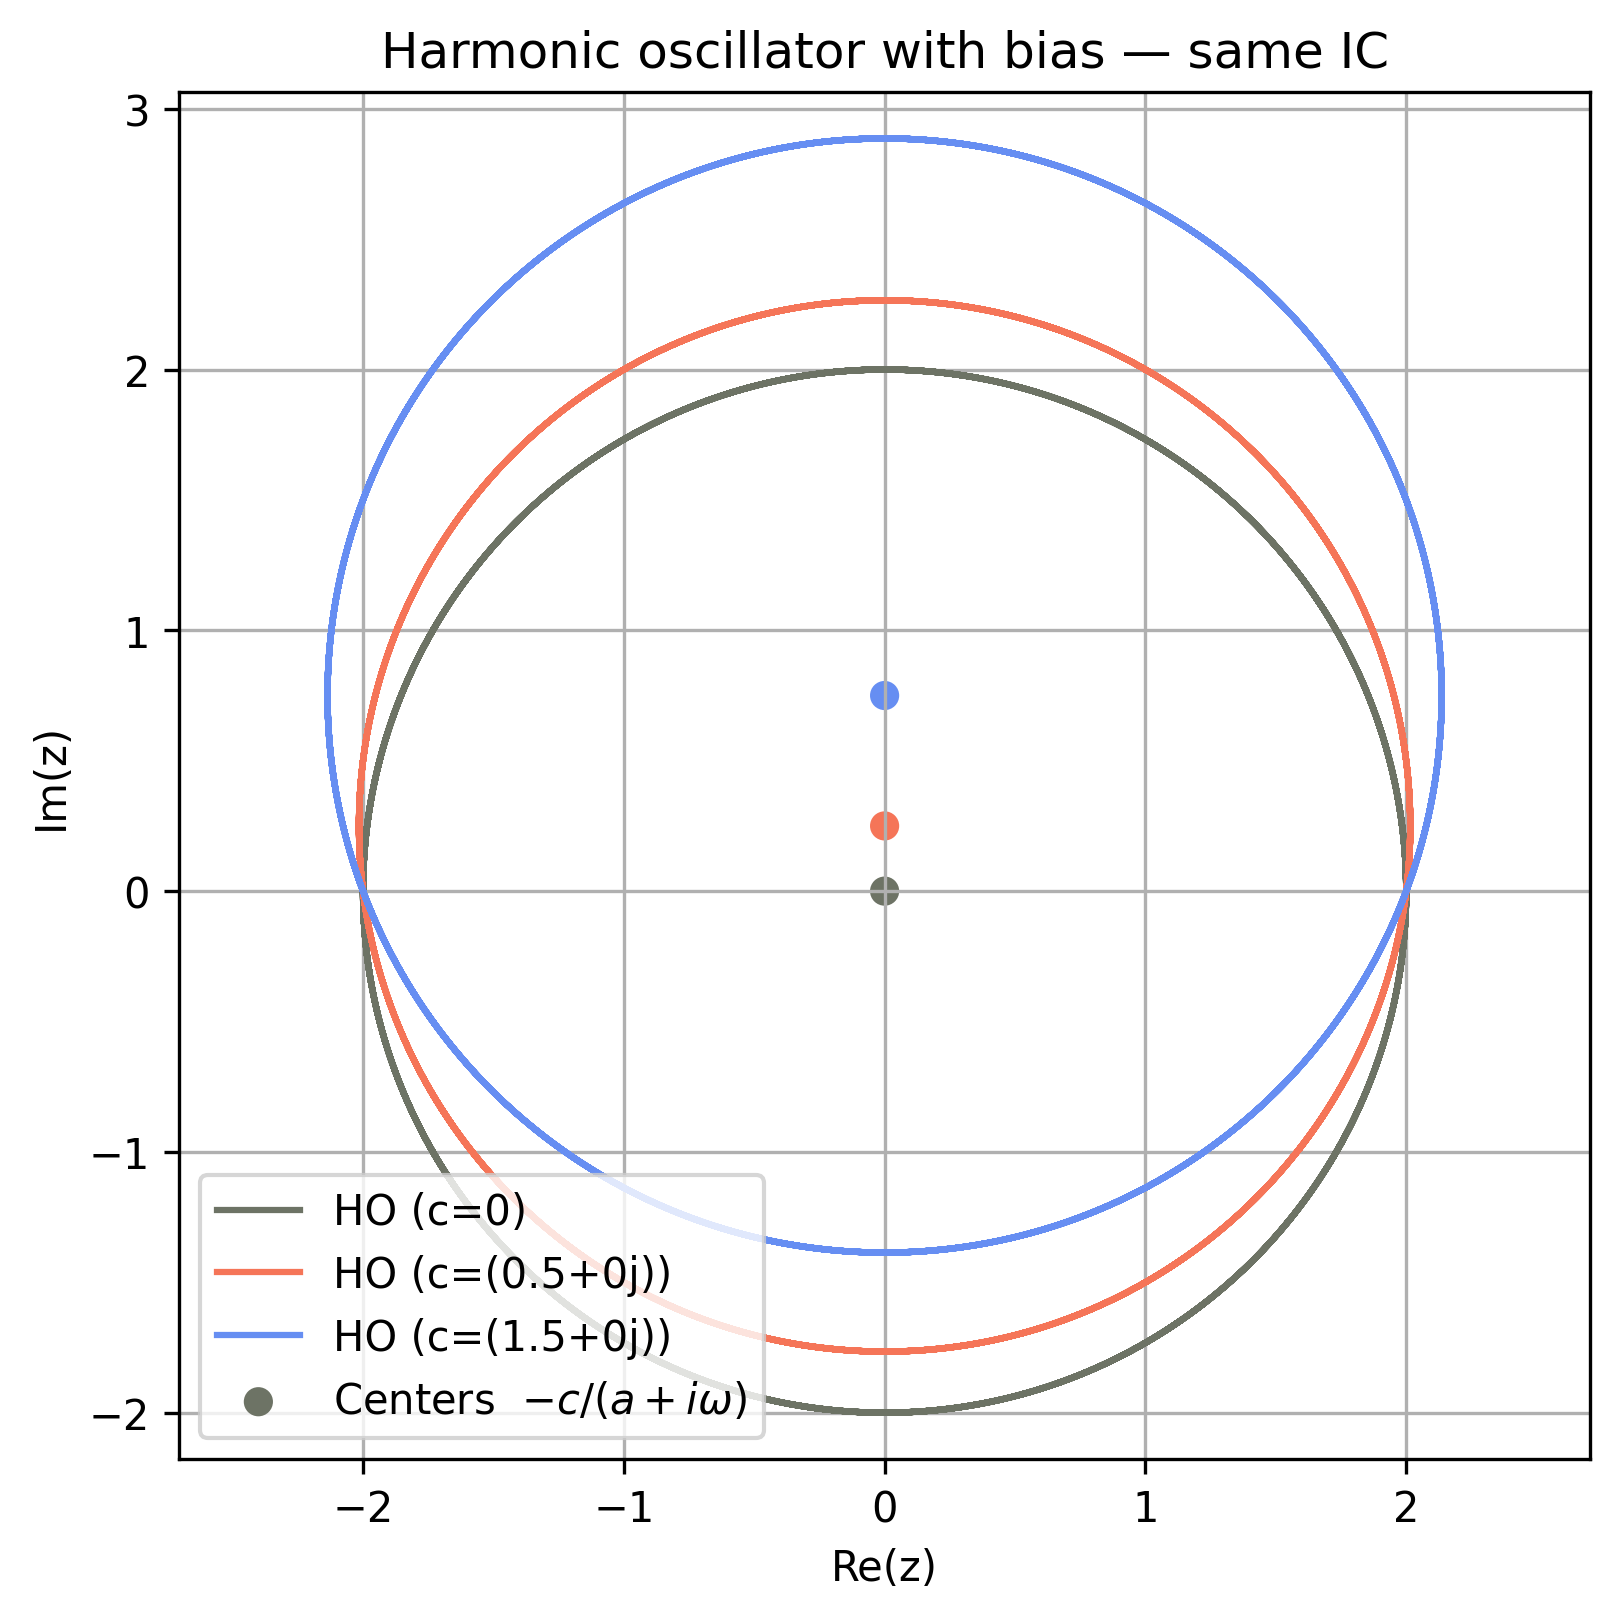
\includegraphics[width=0.48\linewidth]{figures/Figure15.png}
         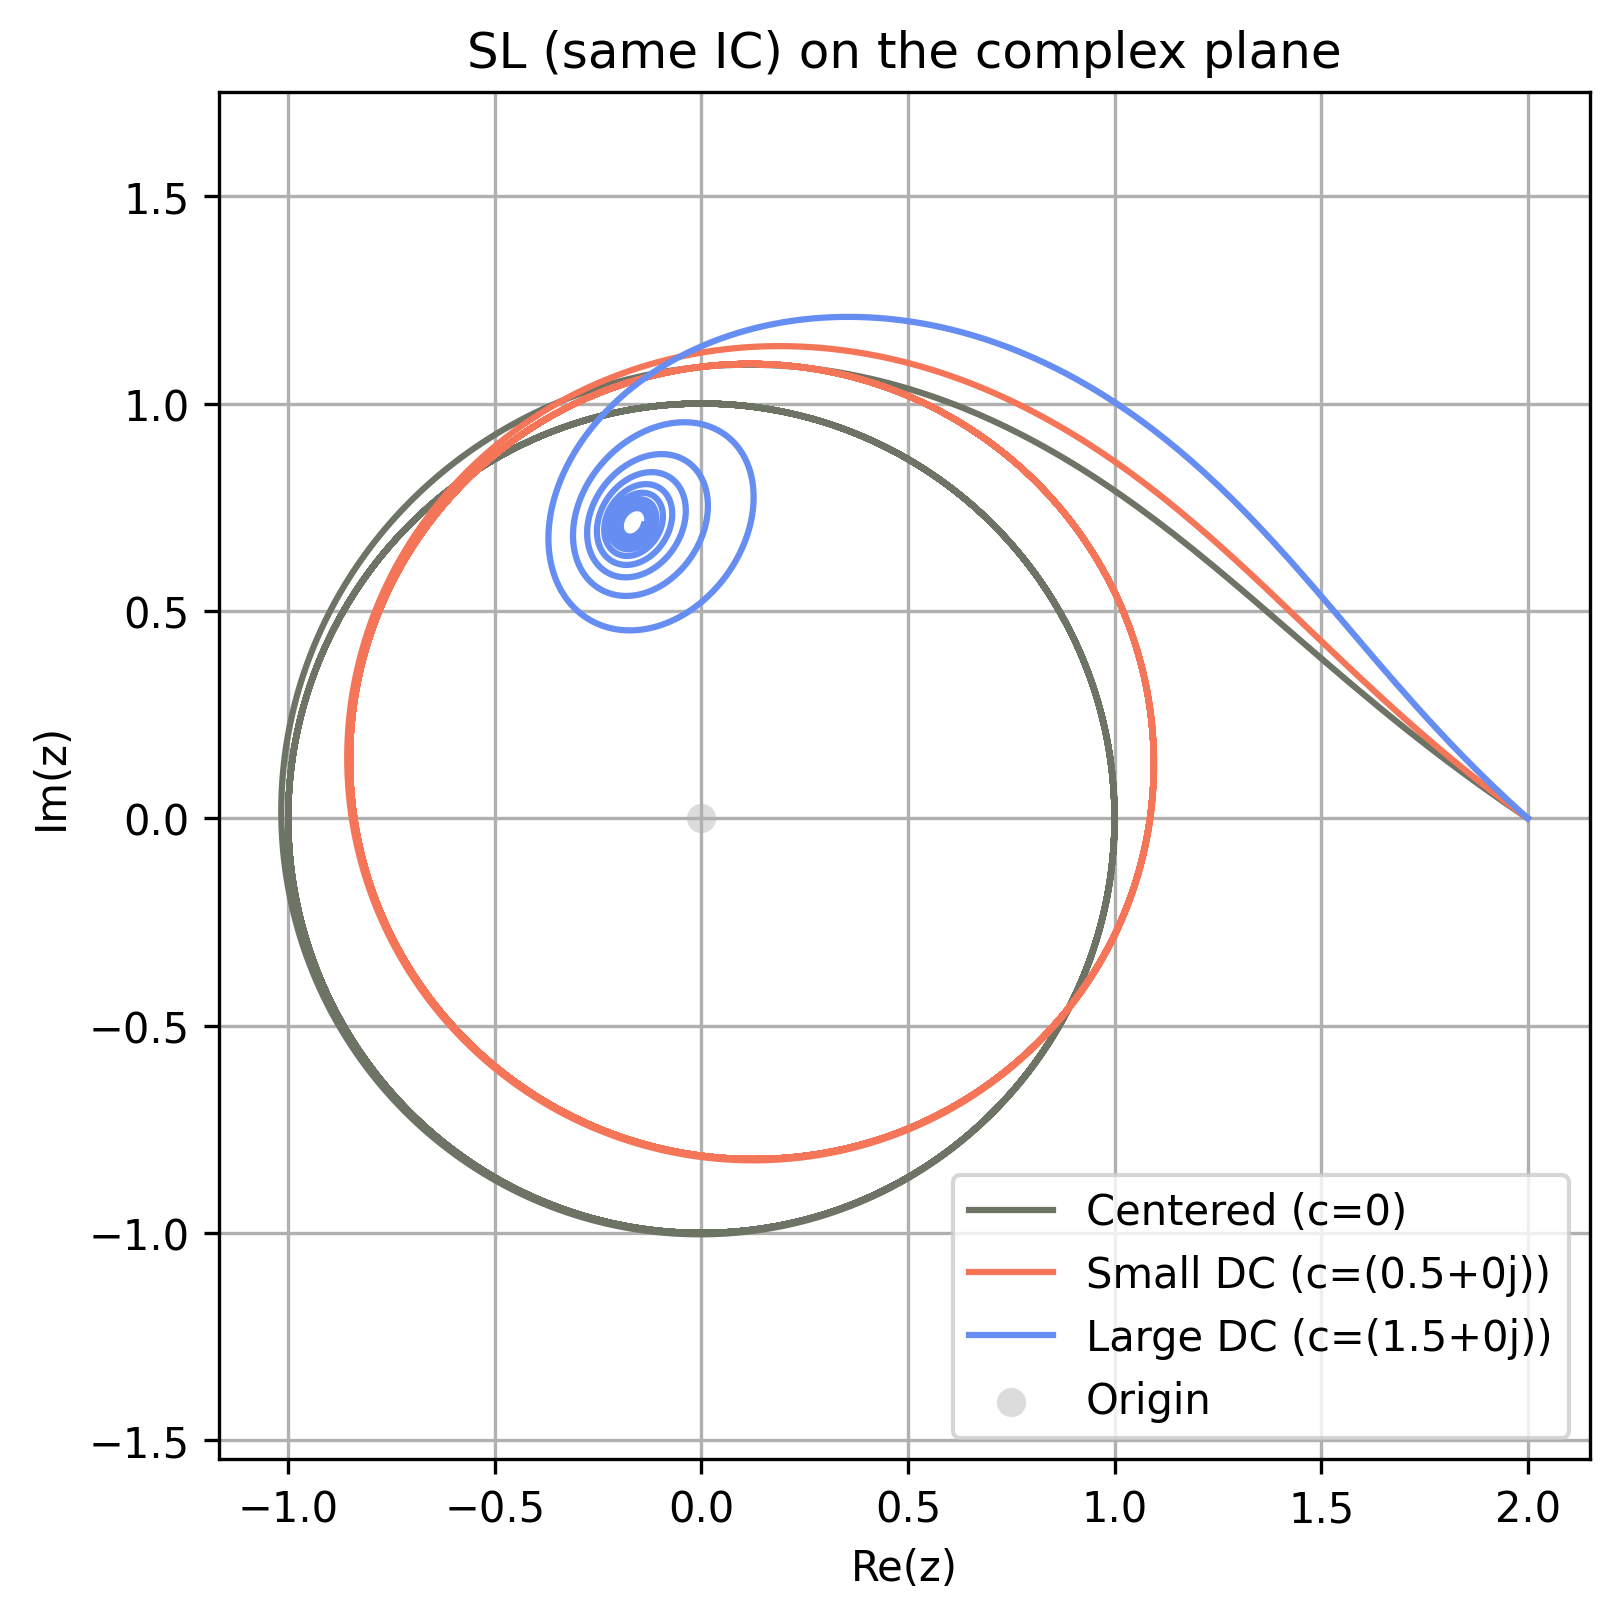
\includegraphics[width=0.48\linewidth]{figures/Figure16.png}

     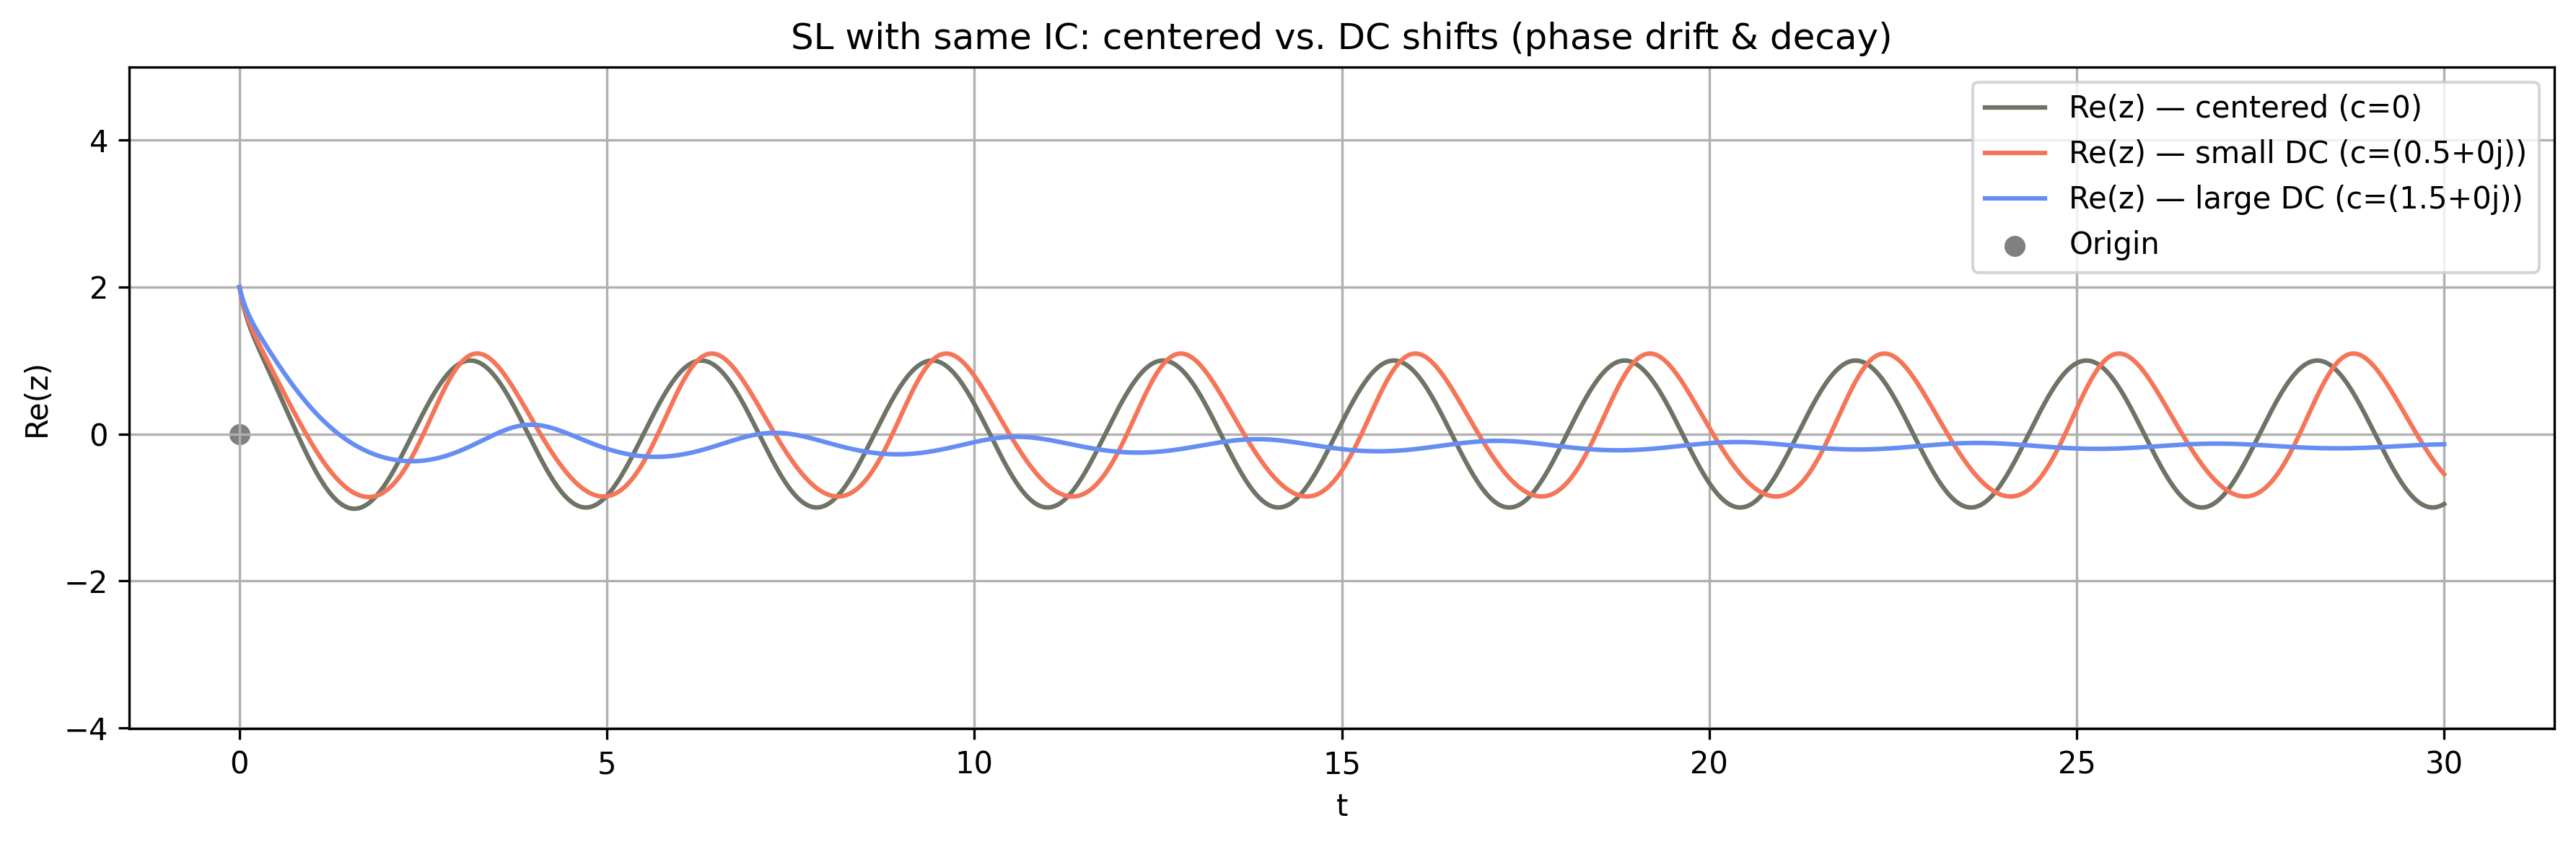
\includegraphics[width=1\linewidth]{figures/Figure17.png}
     \caption{\textbf{Top: Harmonic Oscillator (HO) and Stuart–Landau (SL) with a bias: phase portraits.} Simulations display the effects of a small or larger DC bias offset, which induce frequency and amplitude changes, or destroy the limit cycle in SL while producing simple displacements in HO.
We integrate $\dot z=(\mu+i\omega)z-(g+i\beta)\lvert z\rvert^2 z + c$ with
$\mu=1$, $g=1$, $\omega=2$, $\beta=0$, using RK4 ($\Delta t=0.01$).
Cases: (i) centered SL ($c=0$), (ii) small DC shift ($c=0.5+0i$) yielding a displaced
limit cycle, (iii) large DC shift ($c=2+0i$) leading to convergence to the fixed point. Initial condition for all runs: $z_0=2R_0$ with $R_0=\sqrt{\mu/g}=1$.
Trajectories shown after transients to emphasize the displaced cycle and the decay. \textbf{Bottom: SL time-series overlay.} The three cases are shown, highlighting changes in frequency and amplitude as well as extinction. 
}

     \label{fig:SLtimeseries}
 \end{figure}
 % Figures: https://colab.research.google.com/drive/1qCRZ1M8WsNsB247IG8tB6GSBaRMkIgP-#scrollTo=y35I4EjHynUB

 
 


 
 

However, introducing a constant DC bias to the Stuart–Landau oscillator modifies its equilibrium position, breaks the symmetry, and shifts the critical Hopf bifurcation threshold, thus altering both amplitude and frequency of oscillations (see Figure~\ref{fig:SLtimeseries} for an example). Small biases result in second-order reductions in oscillation amplitude and frequency shifts, whereas sufficiently large DC offsets can completely eliminate the limit cycle. Analytically, this can be described as an imperfect Hopf bifurcation: the effective bifurcation parameter ($\mu$) is renormalized by the DC term, requiring a higher original parameter value to sustain oscillations. Hence, persistent oscillations occur only when the system’s gain overcomes the bias-induced suppression; otherwise, the oscillator settles into a stable equilibrium without oscillations.



 

%%%%%%%%%%%%%%%%%%
\clearpage 
%%%%%%%%%%%%%%%%%%%%%%%%%%%%%


\section{Linear Operators, Green--Laplace Tools, and E-I Oscillations: a Pedagogical View}
\label{app:L-op}

Linear differential operators appear throughout neural modeling (synaptic kinetics, population filters, dendritic cable reductions). A compact way to see why they behave like filters is to write
\[
L[x](t)=u(t),\qquad L=\sum_{k=0}^n a_k\,\partial_t^k,
\]
and study two canonical objects. The \emph{homogeneous} solution \(L[x_h]=0\) reveals the system's natural modes, while the \emph{impulse response} \(h\) solves \(L[h]=\delta\) with \(h(t)=0\) for \(t<0\) and encodes the system's causal memory. If the characteristic polynomial \(p(\lambda)=\sum_{k=0}^n a_k\lambda^k\) factors as \(\prod_i(\lambda-\lambda_i)\) with distinct \(\lambda_i\), then \(x_h(t)=\sum_i c_i e^{\lambda_i t}\). The corresponding \(h(t)\) is also a linear combination of the same exponentials for \(t>0\), pinned by standard continuity conditions at \(t=0\) (all derivatives up to order \(n-2\) are continuous; \(x^{(n-1)}\) jumps by \(1/a_n\))  \cite{StakgoldHolst2011}.

\subsection{Two complementary tools: Laplace and Green}
\paragraph{Laplace viewpoint.}
With zero initial conditions, \(\mathcal{L}\{L[x]\}(s)=P(s)X(s)\) where \(P(s)=\sum_k a_k s^k\). The \emph{transfer function} is \(H(s)=X(s)/U(s)=1/P(s)\). Poles of \(H\) set decay rates, oscillation frequencies, and phase lag. Evaluating on the imaginary axis, \(H(j\omega)\), gives magnitude and phase; the \emph{group delay} is \(\tau_g(\omega)=-\frac{d}{d\omega}\arg H(j\omega)\).

\paragraph{Green (time‑domain) viewpoint.}
Equivalently, the causal Green's function \(G(t,t_0)\) satisfies \(L[G(\cdot,t_0)]=\delta(\cdot-t_0)\) with \(G=0\) for \(t<t_0\). For any input \(u\),
\[
x(t)=\int_{-\infty}^t G(t,t_0)\,u(t_0)\,dt_0=(h*u)(t),\qquad h(t)=G(t,0).
\]
Laplace uses exponentials \(e^{st}\) (an eigenbasis of \(\partial_t\)) to expose poles and phase directly; Green uses time‑localized impulses \(\delta(t-t_0)\) to show how past inputs are weighted and delayed  \cite{StakgoldHolst2011}. Both are the same mathematics seen from two bases.

\subsubsection*{A gentle taxonomy by order (with worked examples)}
For clarity we use \(L=a\,\partial_t+b\) for first order and \(L=m\,\partial_t^2+a\,\partial_t+b\) for second order, with \(m>0\), \(a\ge0\), \(b>0\). When convenient we switch to \(\omega_n\) and \(\zeta\) via \(b/m=\omega_n^2\) and \(a/m=2\zeta\omega_n\).

\paragraph{Zeroth order: memoryless gain.}
\(b\,y=f\Rightarrow h(t)=\frac{1}{b}\delta(t)\). There is no temporal memory.

\paragraph{First order: leaky integrator (and integrator limit).}
\(a\,\dot y+b\,y=f\) has \(h(t)=\frac{1}{a}e^{-(b/a)t}H(t)\). The time constant is \(\tau=a/b\). In Laplace, \(H(s)=1/(a s+b)=(1/b)\,1/(1+s\tau)\), so \(\tau_g(\omega)=\tau/(1+(\omega\tau)^2)\). If \(b=0\), \(h(t)=\frac{1}{a}H(t)\) and \(H(s)=1/(a s)\): an ideal integrator with perfect memory.

\paragraph{Second order: rise--decay, critical, underdamped, and negative damping.}
With \(L=m\,\ddot y+a\,\dot y+b\,y\), the roots
\[
r_{1,2}=\frac{-a\pm\sqrt{a^2-4mb}}{2m}
\]
organize all cases. Overdamped (\(a^2>4mb\)): \(h(t)=\dfrac{e^{r_1 t}-e^{r_2 t}}{m(r_1-r_2)}H(t)\), a difference of decays with a delayed peak. Critical (\(a^2=4mb\)): \(h(t)=(1/m)\,t\,e^{-\frac{a}{2m}t}H(t)\) (the alpha form). Underdamped (\(a^2<4mb\)): writing \(\alpha=\frac{a}{2m}\) and \(\omega_d=\frac{\sqrt{4mb-a^2}}{2m}\),
\[
h(t)=\frac{1}{m\omega_d}e^{-\alpha t}\sin(\omega_d t)\,H(t),
\]
an exponentially damped sinusoid. If \(a<0\) (negative friction) the real part of the poles is positive and the response grows.

\subsection{The synapse as a \emph{forced harmonic oscillator}}
It is perhaps more intuitive to understand synaptic delay and inertia by \emph{recognizing the operator} \(L=m\,\partial_t^2+a\,\partial_t+b\) as the mass-spring-damper driven by a force \(f(t)\):
\[
m\,\ddot y(t)+a\,\dot y(t)+b\,y(t)=f(t).
\]
Apply an impulse \(f=\delta\). The mass first acquires velocity, not displacement; energy shuttles between kinetic and spring energy, and damping removes energy. This automatically produces a \emph{delayed} peak in \(y\): the output must build up after the impulse. The same reasoning holds for the electrical RLC analog. In neural mass models, \(y\) is a postsynaptic potential and \(f\) is the presynaptic drive; the ``mass'' \(m\) summarizes effective inertial storage across coupled first‑order elements, while \(a\) and \(b\) summarize leak and restoring tendencies.

\paragraph{Worked example (critical alpha).}
Choose \(h(t)=A\,a\,t\,e^{-a t}H(t)\). Then \(\mathcal{L}\{h\}(s)=A a/(s+a)^2\) and
\[
(s+a)^2 Y(s)=A a\,\Sigma(s)\quad\Longleftrightarrow\quad (\partial_t+a)^2 y(t)=A a\,\sigma(t).
\]
Thus the alpha kernel \emph{is} the impulse response of a critically damped oscillator driven by the presynaptic input. Its delayed peak illustrates a causal, buffer‑like delay with smoothing, not a noncausal time shift.

\paragraph{Peak time and inertia: how mass slows the response.}
Factor \(L=m(\partial_t+a_r)(\partial_t+a_d)\) with \(a_r+a_d=a/m\) and \(a_r a_d=b/m\). In the overdamped case, \(h(t)=\frac{e^{-a_d t}-e^{-a_r t}}{m(a_r-a_d)}H(t)\) peaks at
\[
t_{\mathrm{peak}}=\frac{1}{a_r-a_d}\ln\!\frac{a_r}{a_d}.
\]
At the double pole \(a_r=a_d=a/(2m)\) one gets \(h(t)=(1/m)\,t\,e^{-\frac{a}{2m}t}\) with \(t_{\mathrm{peak}}=2m/a\). In the underdamped case,
\[
h(t)=\frac{1}{m\omega_d}e^{-\alpha t}\sin(\omega_d t)H(t),\qquad
t_{\mathrm{peak}}=\frac{1}{\omega_d}\arctan\!\frac{\omega_d}{\alpha},
\]
with \(\alpha=\tfrac{a}{2m}\) and \(\omega_d=\tfrac{\sqrt{4mb-a^2}}{2m}\). For fixed \(a,b>0\) and \(m\to\infty\), \(\alpha\to0\), \(\omega_d\sim \sqrt{b/m}\), and \(\arctan(\omega_d/\alpha)\to\pi/2\), hence
\[
t_{\mathrm{peak}}\sim \frac{\pi}{2}\sqrt{\frac{m}{b}}\to\infty.
\]
Inertia therefore \emph{increases} the causal delay. Importantly, the overdamped log formula must not be used once the poles become complex; the underdamped expression governs the peak.
 


\subsection{E--I motifs, Barkhausen conditions, and where the phase lag comes from} \label{app:barkhausen}
A pedagogical route to oscillation is to rewrite the undamped oscillator as a pair of coupled first‑order filters. Let \(z=x+i y\) and consider
\[
\dot z=(a+i\omega)z,\qquad a\ge0,\ \omega>0.
\]
Separating real and imaginary parts gives
\[
\dot x=a x-\omega y,\qquad \dot y=a y+\omega x.
\]
Each equation is a leaky integrator driven by the other in \(90^\circ\) phase. When \(a=0\) the loop produces sustained oscillations; when \(a>0\) the envelope decays as \(e^{-a t}\). This ``push--pull'' view is the simplest template to keep in mind as we turn to E-I populations.

\paragraph{Barkhausen as a phase-gain budget.}
For a feedback loop with transfer \(L(s)\), \textbf{necessary conditions for linear self‑oscillation} at \(\omega_0\) are \(|L(j\omega_0)|=1\) and \(\arg L(j\omega_0)=0^\circ \pmod{360^\circ}\) \cite{vonWangenheim2010}. The phase condition pins \(\omega_0\) by balancing element lags; the magnitude condition pins the product of gains, including the slope \(\kappa\) of the nonlinearity at the bias point. Nonlinear saturation then stabilizes amplitude \cite{AstromMurray2008}.

\paragraph{Wilson--Cowan with first‑order synapses.}
Linearize about a fixed point with slope \(\kappa\) and unit time constants:
\[
\dot{x}=-(1-w_{ee}\kappa)x - w_{ei}\kappa\,y + I_x,\qquad
\dot{y}=-y + w_{ie}\kappa\,x - w_{ii}\kappa\,y.
\]
The E\(\to\)I\(\to\)E loop has
\[
T_{EI}(s)=\frac{w_{ei}w_{ie}\kappa^2}{(s+1)^2},
\]
which can supply up to \(-180^\circ\) of phase---not enough alone to close the loop at a finite \(\omega\). Excitatory self‑coupling adds
\[
T_{EE}(s)=\frac{w_{ee}\kappa}{s+1},
\]
so the characteristic equation \(1-T_{EE}(s)-T_{EI}(s)=0\) can satisfy Barkhausen at some \(\omega_0\). A bias \(I_x\) ensuring \(\kappa>0\) is essential \cite{WilsonCowan1972}. This matches the intuition that two first‑order elements need additional phase (or an explicit transmission delay) to reach \(360^\circ\).

\paragraph{Jansen--Rit with second‑order synapses.}
For the cortical column with second‑order synapses,
\[
\ddot{x}+2a\dot{x}+a^2 x=A a\,\kappa(-w\,y+I_x),\qquad
\ddot{y}+2b\dot{y}+b^2 y=B b\,\kappa(w\,x),
\]
the linearized synapses are band‑pass filters
\[
H_{\mathrm{exc}}(s)=\frac{A a\,\kappa}{(s+a)^2},\qquad
H_{\mathrm{inh}}(s)=\frac{B b\,\kappa}{(s+b)^2}.
\]
The E\(\to\)I\(\to\)E loop transfer
\[
T(s)=-\,w^2\,H_{\mathrm{exc}}(s)\,H_{\mathrm{inh}}(s)
\]
can contribute \(-360^\circ\) of phase on its own, so self‑excitation is \emph{not} required to meet the phase condition. A bias \(I_x\) maintaining \(\kappa>0\) sets \(|T(j\omega_0)|=1\) at the selected frequency  \cite{jansen1995}. Empirically, \(\omega_0\) follows the loop's effective delay, which is controlled by synaptic poles \(a,b\) and any axonal conduction delay.

\paragraph{Information flow and effective loop delay.}
For narrowband loops, each element's phase behaves as \(\varphi_k(\omega)\approx -\omega\,\tau_k\) near resonance, so \(\sum_k \varphi_k(\omega_0)=0^\circ\) implies \(\omega_0 \approx 2\pi n/\tau_{\mathrm{loop}}\), where \(\tau_{\mathrm{loop}}\approx -\sum_k \varphi_k(\omega_0)/\omega_0\). Second‑order synapses provide larger group delay around their passband than single‑pole synapses. This is one reason gamma‑range E-I oscillations arise robustly once the synaptic dynamics are at least second order  \cite{BuzsakiWang2012}.

\paragraph{First-order worked example (frequency response to a sinusoid).}
To fix ideas, solve \(\dot x + a x = e^{j\omega t}\) with \(a>0\). In Laplace,
\[
(s+a)X(s)=\frac{1}{s-j\omega}\quad\Rightarrow\quad
X(s)=\frac{1}{(s+a)(s-j\omega)}.
\]
Partial fractions and inversion give
\[
x(t)=\frac{e^{-a t}}{-(a+j\omega)}+\frac{e^{j\omega t}}{a+j\omega}.
\]
The transient term dies as \(t\to\infty\); the steady state is \(x(t)=H(j\omega)\,e^{j\omega t}\) with \(H(j\omega)=1/(a+j\omega)\). Hence \(|H(j\omega)|=1/\sqrt{a^2+\omega^2}\) and \(\arg H(j\omega)=-\arctan(\omega/a)\), and \(\tau_g(\omega)=a/(a^2+\omega^2)\). This calculation makes explicit how a pole at \(-a\) sets both decay and phase lag.

\paragraph{Time-domain worked example (convolution with an alpha kernel).}
Consider \(h(t)=A a t e^{-a t}H(t)\) and an input \(\sigma(t)\). Then \(y(t)=(h*\sigma)(t)\) and \(\mathcal{L}\{h\}=A a/(s+a)^2\). Multiplication in \(s\)-space becomes
\[
Y(s)=\frac{A a}{(s+a)^2}\,\Sigma(s)\quad\Longleftrightarrow\quad
\left(\partial_t+a\right)^2 y(t)=A a\,\sigma(t),
\]
realizing the second‑order operator directly from the kernel. This is the synaptic analog of driving a critically damped mass-spring-damper.

\subsection*{Pointers for further reading}
A rigorous, operator‑theoretic treatment of \(L[h]=\delta\) and the jump conditions appears in  Stakgold \& Holst (2011)  \cite{StakgoldHolst2011}. For feedback, phase, and the Barkhausen criterion in context see {\AA str\"om \& Murray (2008)} \cite{AstromMurray2008} and the clarification in  vonWangenheim (2010) \cite{vonWangenheim2010}. For neural mass modeling with first‑ and second‑order synapses see  Wilson \& Cowan (1972)  \cite{WilsonCowan1972} and  Jansen \& Rit (1995) \cite{jansen1995}; for conductance‑based synaptic kinetics and canonical PSP shapes see  Destexhe\textit{ et al.} (1994) \cite{destexhe1994}; and for a broader review of E--I mechanisms of cortical rhythms see Buzs\'aki\&Wang (2012)  \cite{BuzsakiWang2012}.


\clearpage
\section{Oscillations, Topology and Simplicity}
\label{app:oscillation}
\noindent
The term \textit{oscillation} is used across mathematics, engineering and neurophysiology, yet each community defines it  differently  (see Table~\ref{tab:osc_types}).  In this section we show how
all views — dynamical systems, spectral tests, and Koopman eigenanalysis share the same core intuition: \textit{an oscillation is present when the data are better explained (or more concisely described) starting from the baseline of circular motion ($S^1$ topology) than by any simpler alternative.} We will formalize this through an algorithmic definition that more or less says "an oscillation is something that essentially goes around a circle". 


An intuitive \textbf{classical definition} is the following.

 
\paragraph{Definition 1.}
\emph{A dynamical variable is said to oscillate when it exhibits sustained, approximately periodic departures around a reference value such that the system returns to a similar state after a characteristic approximate interval $T$ (its period), or, equivalently, at a dominant frequency $f=1/T$.  The repetition can be exact (strictly periodic) or approximate (quasi‑periodic, weakly modulated, or noise‑jittered); what matters is the recognisable cycle pattern.}
 

This phrasing captures the intuition of ``a signal that roughly repeats'' while making explicit (i) the presence of a characteristic timescale and (ii) tolerance for imperfect cycles.




This practical notion—a pattern that \emph{roughly} repeats—is compatible both with modern spectrum‑based detectors and with the dynamical‑systems idea of an attracting limit cycle.  But it can be generalized to include damped behavior:

 
\paragraph{Definition 2.}
\emph{An oscillation is a self‑sustained or externally driven fluctuation that revisits comparable states at quasi‑regular intervals, identifiable either as a closed trajectory in state space or as a narrow‑band spectral peak above the aperiodic background.}
 

This sentence bridges physics, signal processing, and neuroscience, preparing the ground for the algorithmic‑information view developed in the following sections. We revise first the definitions in different sub-fields.






\begin{table}[t!]\small
\centering
\caption{How major fields articulate the notion of oscillation.}
\label{tab:field_views}
\begin{tabular}{p{3.2cm}p{6.5cm}p{4.3cm}} 
\toprule
\textbf{Field} & \textbf{Typical wording} & \textbf{Key nuance} \\
\midrule
Classical physics \& engineering &
``Repetitive or \emph{periodic} variation, typically in time, of a quantity about a central value (often an equilibrium) or between two states.'' \cite{Kreyszig11}  &
Emphasizes small deviations from equilibrium and strictly periodic motion (e.g.\ undamped spring, AC current). \\[4pt]

Non‑linear dynamics / mathematics &
A \emph{periodic orbit} (or \emph{limit cycle}) satisfying $x(t+T)=x(t)$; at least one nearby trajectory spirals into it.\cite{Strogatz1994} &
Formal, coordinate‑free; includes self‑sustained oscillators (Van der Pol, Hodgkin–Huxley) and supports stability analysis. \\[4pt]

Neuroscience &
``Rhythmic or repetitive neural activity observed at all levels of the CNS.''  \cite{Basar13}&
Focus on multi‑scale biological generators; amplitude mainly indexes population synchrony, not a single source. \\[4pt]

Signal processing / spectral view &
``Narrow‑band peak that rises above the aperiodic 1/\emph{f} background in the power spectrum.'' \cite{Donoghue20}&
Detects oscillations without explicit time‑domain periodicity; robust for noisy or burst‑like data. \\
\bottomrule
\end{tabular}
\vspace{-6pt}
\end{table}
%-----------------------------------------------------




\paragraph{Oscillations and the Koopman Operator.}
A \textit{limit cycle} is a closed orbit $\gamma$ of an autonomous ODE to which at least one neighbouring trajectory spirals (stable Floquet multipliers) \cite{Strogatz94}. The system’s intrinsic period $T$ is exact, and, as we explain, next, its Koopman operator possesses an eigenpair $(\psi,\lambda=i\omega)$ whose argument $\theta=\arg\psi$ advances uniformly, embedding the dynamics on the circle $S^{1}$ \cite{Koopman31}.  

Thus,  periodic behavior can be precisely described from the  Koopman operator perspective \cite{Koopman31}. Relaxation oscillators (e.g.\ FitzHugh–Nagumo) fit the same definition but spend long intervals on slow manifolds, producing nonsinusoidal waveforms with rich harmonic content.





This approach fundamentally reframes the analysis. Instead of studying the nonlinear evolution of the system's state vector $\mathbf{x}(t) \in \mathbb{R}^n$ (governed by $\dot{\mathbf{x}} = \mathbf{f}(\mathbf{x})$), the Koopman operator $\mathcal{K}^t$ describes the \textit{linear} evolution of   ``observables'' $g(\mathbf{x})$ (cleverly chosen functions of the state). The operator is defined by how it advances any such function along the system's trajectories: $(\mathcal{K}^t g)(\mathbf{x}_0) = g(\mathbf{x}(t))$, where $\mathbf{x}(t)$ is the flow starting from $\mathbf{x}_0$. The crucial insight is that $\mathcal{K}^t$ is a \textbf{linear operator} acting on the (infinite-dimensional) space of observables, even when the underlying dynamics $\mathbf{f}(\mathbf{x})$ are nonlinear.

Because $\mathcal{K}^t$ is linear, we can use spectral methods. For a limit cycle, the operator's \textit{infinitesimal generator} $L$ (where $\mathcal{K}^t = e^{Lt}$) possesses an eigenpair $(\psi, \lambda=i\omega)$ corresponding to the system's fundamental frequency $\omega = 2\pi/T$. This special observable $\psi$, the \textbf{Koopman eigenfunction}, evolves simply in time: $\psi(\mathbf{x}(t)) = (\mathcal{K}^t \psi)(\mathbf{x}_0) = e^{\lambda t} \psi(\mathbf{x}_0) = e^{i\omega t} \psi(\mathbf{x}_0)$. Consequently, its argument $\theta=\arg\psi$ advances uniformly ($\theta(t) = \theta_0 + \omega t$), embedding the complex, multi-dimensional dynamics onto a simple rotation on the circle $S^{1}$. Relaxation oscillators (e.g.\ FitzHugh–Nagumo) fit the same definition, but their corresponding eigenfunctions $\psi$ are more complex (capturing all the harmonics), resulting in nonsinusoidal waveforms.

It is important to clarify what the eigenfunction $\psi$ represents. It is a special \textbf{observable}, meaning it is a function of the state vector, $\psi(\mathbf{x})$, that maps the $n$-dimensional state space (where the dynamics are nonlinear) to the complex plane $\mathbb{C}$ (where the dynamics are linear). Its special property is that when evaluated \textit{along} a trajectory $\mathbf{x}(t)$, its value evolves with perfect simplicity according to $\psi(\mathbf{x}(t)) = e^{i\omega t}\psi(\mathbf{x}_0)$.

%Crucially, one must distinguish the function $\psi(\mathbf{x})$---which is a static, complex-valued map on the state space---from its \textit{evolution in time}, $\psi(\mathbf{x}(t))$. The function $\psi(\mathbf{x})$ itself is generally not periodic. 

In essence, $\psi$ acts as a ``magic'' coordinate transformation. While the state $\mathbf{x}(t)$ traces a complex orbit, the scalar observable $\psi(\mathbf{x}(t))$ simply rotates in the complex plane at a constant frequency $\omega$. The level sets of its phase, $\theta = \arg \psi(\mathbf{x})$, are the system's \textbf{isochrons}: surfaces of points in the state space that all share the same asymptotic phase on the limit cycle.

\paragraph{Koopman perspective as compression.}
Finding an eigenfunction $\psi$ with generator eigenvalue $ \lambda=i\omega$ represents a form of compression. Once this function $\psi$ is known, the full $n$‑dimensional trajectory $\mathbf x(t)$ can be encoded (losslessly near the attractor) by a single complex phase variable $\psi(\mathbf{x}(t))$, or separated into its phase $\theta(t)=\arg\psi(\mathbf x(t))$ and amplitude $r(t)=|\psi(\mathbf x(t))|$ \cite{Koopman31}. In effect, the Koopman transform finds a ``magic'' coordinate system $\psi$ in which the nonlinear dynamics become simple linear rotation. It replaces a complex waveform with uniform rotation on $S^{1}$, turning geometry into a one‑line program: \texttt{output $r(t) \cdot \cos(\theta(t))$}.

%\paragraph{Connection to Diffeomorphisms and Lie Groups.}  The flow of the dynamical system, $\Phi^t: M \to M$, maps an initial state $\mathbf{x}_0$ to its position at time $t$, $\mathbf{x}(t) = \Phi^t(\mathbf{x}_0)$. For a smooth vector field $\mathbf{f}$, this flow $\Phi^t$ is a \textit{diffeomorphism} (a smooth, invertible map with a smooth inverse). The set of all such flows $\{\Phi^t\}_{t \in \mathbb{R}}$ forms a \textit{one-parameter group} under composition: $\Phi^t \circ \Phi^s = \Phi^{t+s}$. This group is a subgroup of the full \textit{infinite-dimensional Lie group} of all diffeomorphisms of the state space $M$, denoted $\text{Diff}(M)$.

%The Koopman operator $\mathcal{K}^t$ is the \textit{pullback} (or composition) operator induced by this flow. It is defined as $(\mathcal{K}^t g) = g \circ \Phi^t$, or $(\mathcal{K}^t g)(\mathbf{x}) = g(\Phi^t(\mathbf{x}))$. The Koopman operator family $\{\mathcal{K}^t\}$ also forms a one-parameter group, $(\mathcal{K}^t \circ \mathcal{K}^s)g = g \circ \Phi^s \circ \Phi^t = g \circ \Phi^{s+t} = \mathcal{K}^{t+s}g$. Crucially, this provides a \textbf{linear representation} of the (nonlinear) flow group $\{\Phi^t\}$ on the (infinite-dimensional, linear) space of observable functions.

%This relationship extends to their generators. The generator of the flow group $\{\Phi^t\}$ is the vector field $\mathbf{f}$ itself, which is an element of the Lie algebra $\text{Vect}(M)$ (the space of vector fields on $M$). The generator of the Koopman group $\{\mathcal{K}^t\}$ is the operator $L$. This generator $L$ is precisely the \textbf{Lie derivative} with respect to the vector field $\mathbf{f}$, $L = L_{\mathbf{f}}$, which acts on observables $g$ as $Lg = (\mathbf{f} \cdot \nabla) g$. Thus, the Koopman framework ``lifts" the nonlinear dynamics from the state space $M$ to a linear representation on a function space, where the generator is the Lie derivative.



\paragraph{Signal‑processing criteria}.
In experimental neurophysiology, oscillations are said to  be  \textit{detected} according to some criteria.  
Two widely used operational rules are  
(i) the BOSC power\,+\,duration test \cite{Whitten11} and  
(ii) spectral parameterisation (``FOOOF'') that labels any narrow‑band bump lying above the aperiodic 1/\emph{f} background as oscillatory \cite{Donoghue20}.  
Both are statistical surrogates for asking whether a periodic template explains the data substantially better than a broadband model. Spectral peaks are suggestive of reduced entropy or increased compressibility.


Table \ref{tab:osc_types} aligns the main modeling traditions—from classical limit–cycle theory to modern information–theoretic views—while the text links them through the common intuition that  \textit{circular motion in an abstract coordinate revealed by compression}.



Next, we discuss the formalization of this intuition and  generalization of the above definitions using the language of algorithmic information theory and compression (AIT)\cite{cover_elements_2006}.



%--------------------------------------------------------------------
\begin{table}[t!]
\centering
\caption{Representative oscillator types and the lenses through which they are defined or detected.}
\label{tab:osc_types}
\begin{tabular}{p{3.3cm}p{4.5cm}p{3.5cm}p{3.3cm}}
\toprule
\textbf{Oscillation class} & \textbf{Canonical models} & \textbf{Koopman lens } & \textbf{Spectral lens}\\
\midrule
\textbf{Limit cycle} & Harmonic oscillator; Van der Pol \cite{VanDerPol26}; Stuart–Landau \cite{Stuart58} & $\lambda = i\omega$ (purely imaginary) & Dirac comb (infinitely sharp harmonics)  \\
\addlinespace[2pt]
\textbf{Relaxation oscillator} & FitzHugh–Nagumo \cite{FitzHugh61}; Morris–Lecar \cite{Morris81} & $\lambda  = i\omega$ plus strong higher harmonics &   ($\uparrow$ bandwidth) \\
\addlinespace[2pt]
\textbf{Damped spiral / ring‑down} & Linear focus; LCR circuits & $\lambda = \alpha + i\omega,\; \alpha < 0$ & Lorentzian PSD peak (width $\sim|\alpha|$)  \\
\addlinespace[2pt]
\textbf{Noise‑sustained quasi‑cycle} & Linear focus $+$ stochastic drive \cite{McKane05} & Same $\lambda$ as above, noise keeps $| \psi|>0$ & Finite‑width peak  \\
\bottomrule
\end{tabular}\\[2pt]
\end{table}
%--------------------------------------------------------------------
\subsection*{Algorithmic‑information definition}

Algorithmic Information Theory (AIT) takes a computational perspective and quantifies the information content of \emph{individual} objects via computation rather than probability. 
For a binary string $x$, the (prefix) Kolmogorov complexity $K_U(x)$ is defined as the length (in bits) of the shortest program $p$ that makes a fixed universal prefix-free Turing machine $U$ output $x$ and halt,
\begin{equation}
K_U(x) = \min_{p \in \{0,1\}^*} \{\, |p| \; : \; U(p) = x \,\}.
\end{equation}
By the \emph{Kolmogorov invariance theorem}, $K_U(x)$ depends on the choice of $U$ only up to an additive constant independent of $x$, and one typically writes $K(x)$. 
The conditional version $K(x\,|\,y)$ is defined analogously (what is the complexity of $x$ if we know $y$?). 
Kolmogorov complexity is uncomputable (though upper-semicomputable) and provides the foundation for formal notions of randomness, structure, and the ultimate limits of lossless compression.
For a detailed treatment, see classical textbooks on algorithmic information theory \cite{cover_elements_2006,li_applications_2007}.


\paragraph{Compressing data from an oscillator.} Let $x_{1:N}$ be the measured signal.  
Our compressor stores the following program: 
(i) a periodic template $u_{1:T}$ with some frequency (U1 limit‑cycle model with nonlinear mapping / Koopman operator, $K_{\text{LC}}$ bits) and  
(ii) a residual code $e$ (modulation, burst gaps,  remaining error / noise) of length $K_e$.  
If
\[
K_{\text{LC}} + K_{\text{e}} \;\; \ll \;\; L_{\text{raw}} \; ,
\]
where $L_{\text{raw}}$ is the length of a generic lossless code (e.g.\ LZ‑77 or Huffman on the empirical alphabet), we say the sequence \emph{contains an oscillation}.  
No reference model is required—the gain is measured against the unstructured data description.

\paragraph{Relation to Koopman.}
The ideal template $u_{1:T}$ corresponds to one traversal of the Koopman phase; storing $\theta_0$ and $\omega$ plus a small update map for $r$ therefore yields the shortest program in the Kolmogorov sense.  
Thus, the ``kernel'' of every oscillator is circular motion, and oscillation = substantial description‑length reduction via an $S^{1}$ code.

\paragraph{Generative view.} We say that a dataset contains an oscillation if it can be Lie-generated by the U(1) group. In other words, the latent space coordinate of the generative model is $\theta \in S^1$. The generative  (compressive) model is of the form data = $M(\theta)$ + noise.
 In AIT, an \textit{algorithmic agent} would declare, \textit{``An oscillation is a detected pattern: a signal that approximately repeats."}  A bit more precisely, a dynamical dataset is said to contain an oscillation when a periodic‑template model (program) compresses the data significantly better than any model that lacks periodic structure.  But we can be more precise using the notion of Lie-generated model \cite{ruffiniAITFoundationsStructured2022,ruffiniStructuredDynamicsAlgorithmic2023}: 


\begin{tcolorbox}[colback=gray!12,colframe=gray!12,enlarge left by=0mm,
  boxrule=0pt,sharp corners]
  \textbf{Propoed definition:}  A dataset is said to represent an oscillation when it can be most succinctly Lie-generated from a representation of U1 plus noise.
\end{tcolorbox}
 Topologically, every limit cycle is a circle. Hence, a compression algorithm will naturally start from the specification of the circle (the U1 group) plus a mapping and corrections. Or, more generally, from the specification of a U1 invariant object.  We analyze this further in the next section. 


 
\subsection*{U1 and the topology of the Stuart-Landau equation}
\label{app:limitcycles}
The origin of U1 and the topology of $S^1$ can be unearthed cleanly in the case of the Hopf bifurcation.

Oscillatory dynamics---limit cycles in the phase space of a dynamical system---play a central role in modeling neural population activity and other biological rhythms. 


We begin this journey with the simplest possible oscillator: a \emph{phase clock}, defined by a variable $\theta(t)$ advancing at constant rate $\dot{\theta} = \omega$. This system has no amplitude, only phase, and its trajectory lies on a circle. Importantly, it enjoys continuous phase-shift invariance: the dynamics are unchanged under $\theta \to \theta + \phi$, for any fixed phase offset $\phi$. This is the defining symmetry of the circle group $U(1)$---the group of rotations in the plane.

The next natural step introduces amplitude: the \emph{harmonic oscillator} (HO). It describes circular motion in two dimensions at a fixed radius, and takes the form
\[
\dot z = i\omega z,
\]
in complex notation. The solution is $z(t) = z_0 e^{i\omega t}$, and the motion traces a perfect circle in phase space. Again, we see the same $U(1)$ phase symmetry: multiplying a solution by $e^{i\phi}$ simply rotates the initial condition, leaving the dynamics invariant. However, the amplitude $|z|$ remains constant---there is no mechanism for growth, decay, or saturation. Any initial amplitude persists indefinitely, and the system is neutrally stable.

Real-world oscillators behave differently. In practice, oscillations may grow or decay, but often they settle onto a stable limit cycle: a rhythm of fixed amplitude that persists after transients decay. To capture this, we must go beyond the linear HO and introduce nonlinearities that regulate amplitude. Consider adding smooth perturbations to the harmonic oscillator:
\[
\dot z = (\mu + i\omega)\,z + F(z,\bar z),
\]
where $F$ contains higher-order nonlinear terms. The goal is to find the simplest nonlinear correction that leads to amplitude saturation---i.e., to a self-limiting oscillator.

To identify the relevant terms, we use tools from normal form theory: center manifold reduction followed by a near-identity change of coordinates \cite{guckenheimer2013nonlinear,kuznecovElementsAppliedBifurcation1995}. These procedures systematically eliminate all \emph{non-resonant} terms---i.e., terms whose angular dependence does not match that of the linear part and thus oscillate out of phase. At third order, the only resonant term that survives the coordinate transformation process is
\[
F(z,\bar z) = - (g + i\beta)\,|z|^2 z.
\]
All other cubic combinations, such as $z^2$ or $\bar z^2$, are non-resonant and can be removed by choosing proper coordinates. The resulting simplified system is the \emph{Stuart-Landau equation}:
\[
\dot z = (\mu + i\omega)\,z - (g + i\beta)\,|z|^2 z,
\]
which describes a self-excited oscillator: for $\mu > 0$, the amplitude $r = |z|$ grows until it stabilizes at $r = \sqrt{\mu/g}$; for $\mu < 0$, oscillations decay to rest. The equation also governs the phase evolution $\theta = \arg(z)$, with $\dot\theta = \omega - \beta r^2$.

\paragraph{The emergence of \texorpdfstring{$U(1)$}{U(1)} symmetry.}
At no point did we assume that the nonlinear system was $U(1)$-symmetric. We began with a generic perturbation of the harmonic oscillator. However, after applying normal form reduction, we find that only \emph{resonant} terms cannot be removed—those that transform under rotation in the same way as the linear term. At third order, the only such term is $|z|^2 z$, which happens to be $U(1)$-covariant. All non-covariant terms are eliminated by a coordinate transformation. Thus, the $U(1)$ symmetry of the Stuart-Landau equation emerges \emph{as a consequence} of the reduction process.  But the ultimate origin of this is topological: limit cycles are topological circles, and the ``simplest" description of a cycle, the ``platonic" cycle is a circle.

\paragraph{Cohomology and emergence of resonant terms.} The emergence of the Stuart-Landau normal form from generic nonlinear oscillators can thus be understood by appealing to topology and cohomology. Near a Hopf bifurcation, the system dynamics collapse onto a limit cycle—a smooth, closed loop in phase space that is topologically equivalent to the circle, $S^1$.   The circle $S^1$ is a simple but topologically rich space. It admits a special type of 1-form, $d\theta$, which is \emph{closed}, meaning that its exterior derivative vanishes ($d(d\theta)=0$), but it is not \emph{exact}, meaning it cannot be expressed globally as the differential of any smooth scalar function. Exact forms represent trivial cohomological classes because they can be integrated globally, whereas closed but non-exact forms represent fundamental, nontrivial topological features. This distinction is captured by the nontrivial first de Rham cohomology of the circle, $
H^1_{\mathrm{dR}}(S^1)\cong \mathbb{R}.
$
To eliminate nonlinear terms near the bifurcation, we perform a near-identity coordinate transformation, attempting to remove as many nonlinear perturbations as possible. Specifically, we consider coordinate changes of the form
\[
z \mapsto z + H(z,\bar{z}),
\]
and ask whether a given nonlinear perturbation $F(z,\bar z)$ can be eliminated. Under the linearized dynamics, characterized by pure rotations with frequency $\omega$, the infinitesimal rotation operator naturally arises as the Lie derivative,
\[
\mathcal{L}_0 = \omega \frac{\partial}{\partial \theta},
\]
which describes how functions and vector fields vary as we rotate around the limit cycle. Formally, solving the normal-form reduction involves repeatedly solving equations of the form
\[
\mathcal{L}_0 H = F - N,
\]
where $F$ is the nonlinear perturbation we start with, $N$ is the simplified normal form we desire, and $H$ is the coordinate change we seek to perform.

The crucial point is that certain nonlinear terms are \emph{resonant}: their angular frequency exactly matches the natural rotation frequency $\omega$. Such resonant terms belong to the kernel (null space) of the Lie derivative $\mathcal{L}_0$. Geometrically, these terms correspond precisely to closed but non-exact forms on $S^1$. Cohomologically, resonant terms represent nontrivial elements of the first cohomology group associated with $\mathcal{L}_0$:
\[
H^1(\mathcal{L}_0)=\frac{\ker \mathcal{L}_0}{\mathrm{im}\,\mathcal{L}_0}\cong H^1_{\mathrm{dR}}(S^1)\cong \mathbb{R}.
\]
Therefore, no smooth local coordinate transformation (which can only add exact forms) can eliminate these resonant terms, and thus they constitute genuine cohomological obstructions.

At cubic order, this resonance condition selects uniquely the term $|z|^2 z$, ensuring its survival after normal-form reduction. Similarly, higher-order resonant terms take the general form $|z|^{2m} z$, while non-resonant terms oscillate out of synchrony with the natural rotation and lie within the image of $\mathcal{L}_0$. Thus, these non-resonant terms correspond to exact forms and can always be removed by appropriate coordinate changes.

This topological argument generalizes straightforwardly to higher-order nonlinear terms, ensuring that at every odd order only terms of the form $|z|^{2m} z$ survive. Hence, the general normal form near a Hopf bifurcation is universally structured as
\[
\dot z = (\mu+i\omega)z + z\,g(|z|^2),
\]
a direct consequence of the underlying circle geometry and its associated cohomological constraints.






%%%%%%%%%%%%%%%%%%%%%%%%%%%%%%%%%%%%%%%%%%%%%%%%%%
    

